\chapter{Git}
\section{Introduction}
\section{Everyday GIT With 20 Commands Or So}
Individual Developer (Standalone) commands are essential for anybody who makes
a commit, even for somebody who works alone.  If you work with other people,
you will need commands listed in the [Individual Developer (Participant)
section as well.  People who play the Integrator role need to learn some more
commands in addition to the above.  [Repository Administration] commands are
for system administrators who are responsible for the care and feeding of git
repositories.

\subsection{Individual Developer (Standalone)}
A standalone individual developer does not exchange patches with other people,
and works alone in a single repository, using the following commands.

\begin{itemize}
\setlength{\itemsep}{0cm}
\setlength{\parskip}{0cm}
\item git-init(1) to create a new repository.
\item git-show-branch(1) to see where you are.
\item git-log(1) to see what happened.
\item git-checkout(1) and git-branch(1) to switch branches.
\item git-add(1) to manage the index file.
\item git-diff(1) and git-status(1) to see what you are in the middle of doing.
\item git-commit(1) to advance the current branch.
\item git-reset(1) and git-checkout(1) (with pathname parameters) to undo changes.
\item git-merge(1) to merge between local branches.
\item git-rebase(1) to maintain topic branches.
\item git-tag(1) to mark known point.
\end{itemize}

Examples:\\
\lstset{basicstyle=\scriptsize, numbers=none, captionpos=b, tabsize=4}
\begin{lstlisting}[caption=Use a tarball as a starting point for a new repository,language={bash},
breaklines=true,label=lst:useatarballasastartingpointforanewrepository]
$ tar zxf frotz.tar.gz
$ cd frotz
$ git init
$ git add . <1>
$ git commit -m "import of frotz source tree."
$ git tag v2.43 <2>
\end{lstlisting}

\begin{enumerate}
\setlength{\itemsep}{0cm}
\setlength{\parskip}{0cm}
\item add everything under the current directory.
\item make a lightweight, unannotated tag.
\end{enumerate}

\lstset{basicstyle=\scriptsize, numbers=none, captionpos=b, tabsize=4}
\begin{lstlisting}[caption=Create a topic branch and develop,language={bash},
breaklines=true,label=lst:createatopicbranchanddevelop]
$ git checkout -b alsa-audio <1>
$ edit/compile/test
$ git checkout -- curses/ux_audio_oss.c <2>
$ git add curses/ux_audio_alsa.c <3>
$ edit/compile/test
$ git diff HEAD <4>
$ git commit -a -s <5>
$ edit/compile/test
$ git reset --soft HEAD^ <6>
$ edit/compile/test
$ git diff ORIG_HEAD <7>
$ git commit -a -c ORIG_HEAD <8>
$ git checkout master <9>
$ git merge alsa-audio <10>
$ git log --since='3 days ago' <11>
$ git log v2.43.. curses/ <12>
\end{lstlisting}

\begin{enumerate}
\setlength{\itemsep}{0cm}
\setlength{\parskip}{0cm}
\item create a new topic branch.
\item revert your botched changes in curses/ux\_audio\_oss.c.
\item you need to tell git if you added a new file; removal and modification
will be caught if you do git commit -a later.
\item to see what changes you are committing.
\item commit everything as you have tested, with your sign-off.
\item take the last commit back, keeping what is in the working tree.
\item look at the changes since the premature commit we took back.
\item redo the commit undone in the previous step, using the message you
originally wrote.
\item switch to the master branch.
\item merge a topic branch into your master branch.
\item review commit logs; other forms to limit output can be combined and
include --max-count=10 (show 10 commits), --until=2005-12-10, etc.
\item view only the changes that touch what’s in curses/ directory, since v2.43
tag.
\end{enumerate}

\subsection{Individual Developer (Participant)}
A developer working as a participant in a group project needs to learn how to
communicate with others, and uses these commands in addition to the ones needed
by a standalone developer.

\begin{itemize}
\setlength{\itemsep}{0cm}
\setlength{\parskip}{0cm}
\item git-clone(1) from the upstream to prime your local repository.
\item git-pull(1) and git-fetch(1) from "origin" to keep up-to-date with the
upstream.
\item git-push(1) to shared repository, if you adopt CVS style shared
repository workflow.
\item git-format-patch(1) to prepare e-mail submission, if you adopt Linux
kernel-style public forum workflow.
\end{itemize}

\subsubsection{Clone the upstream and work on it. Feed changes to upstream.}
\lstset{basicstyle=\scriptsize, numbers=none, captionpos=b, tabsize=4}
\begin{lstlisting}[caption=,language={bash},
breaklines=true,label=lst:]
$ git clone git://git.kernel.org/pub/scm/.../torvalds/linux-2.6 my2.6
$ cd my2.6
$ edit/compile/test; git commit -a -s <1>
$ git format-patch origin <2>
$ git pull <3>
$ git log -p ORIG_HEAD.. arch/i386 include/asm-i386 <4>
$ git pull git://git.kernel.org/pub/.../jgarzik/libata-dev.git ALL <5>
$ git reset --hard ORIG_HEAD <6>
$ git gc <7>
$ git fetch --tags <8>
\end{lstlisting}

\begin{enumerate}
\setlength{\itemsep}{0cm}
\setlength{\parskip}{0cm}
\item repeat as needed.
\item extract patches from your branch for e-mail submission.
\item git pull fetches from origin by default and merges into the current
branch.
\item immediately after pulling, look at the changes done upstream since last
time we checked, only in the area we are interested in.
\item fetch from a specific branch from a specific repository and merge.
\item revert the pull.
\item garbage collect leftover objects from reverted pull.
\item from time to time, obtain official tags from the origin and store them under .git/refs/tags/.
\end{enumerate}

\subsubsection{Push into another repository.}
\lstset{basicstyle=\scriptsize, numbers=none, captionpos=b, tabsize=4}
\begin{lstlisting}[caption=,language={bash},
breaklines=true,label=lst:]
satellite$ git clone mothership:frotz frotz <1>
satellite$ cd frotz
satellite$ git config --get-regexp '^(remote|branch)\.' <2>
remote.origin.url mothership:frotz
remote.origin.fetch refs/heads/*:refs/remotes/origin/*
branch.master.remote origin
branch.master.merge refs/heads/master
satellite$ git config remote.origin.push \
           master:refs/remotes/satellite/master <3>
satellite$ edit/compile/test/commit
satellite$ git push origin <4>

mothership$ cd frotz
mothership$ git checkout master
mothership$ git merge satellite/master <5>
\end{lstlisting}

\begin{enumerate}
\setlength{\itemsep}{0cm}
\setlength{\parskip}{0cm}
\item mothership machine has a frotz repository under your home directory;
clone from it to start a repository on the satellite machine.
\item clone sets these configuration variables by default. It arranges git pull
to fetch and store the branches of mothership machine to local remotes/origin/*
remote-tracking branches.
\item arrange git push to push local master branch to remotes/satellite/master
branch of the mothership machine.
\item push will stash our work away on remotes/satellite/master remote-tracking
branch on the mothership machine. You could use this as a back-up method.
\item on mothership machine, merge the work done on the satellite machine into
the master branch.
\end{enumerate}

\subsubsection{Branch off of a specific tag.}
\lstset{basicstyle=\scriptsize, numbers=none, captionpos=b, tabsize=4}
\begin{lstlisting}[caption=,language={bash},
breaklines=true,label=lst:]
$ git checkout -b private2.6.14 v2.6.14 <1>
$ edit/compile/test; git commit -a
$ git checkout master
$ git format-patch -k -m --stdout v2.6.14..private2.6.14 |
  git am -3 -k <2>
\end{lstlisting}

\begin{enumerate}
\setlength{\itemsep}{0cm}
\setlength{\parskip}{0cm}
\item create a private branch based on a well known (but somewhat behind) tag.
\item forward port all changes in private2.6.14 branch to master branch without a formal "merging".
\end{enumerate}

\subsection{Integrator}
A fairly central person acting as the integrator in a group project receives
changes made by others, reviews and integrates them and publishes the result
for others to use, using these commands in addition to the ones needed by
participants.
\begin{itemize}
\setlength{\itemsep}{0cm}
\setlength{\parskip}{0cm}
\item git-am(1) to apply patches e-mailed in from your contributors.
\item git-pull(1) to merge from your trusted lieutenants.
\item git-format-patch(1) to prepare and send suggested alternative to contributors.
\item git-revert(1) to undo botched commits.
\item git-push(1) to publish the bleeding edge.
\end{itemize}

A typical git day.
\lstset{basicstyle=\scriptsize, numbers=none, captionpos=b, tabsize=4}
\begin{lstlisting}[caption=,language={bash},
breaklines=true,label=lst:]
$ git status <1>
$ git show-branch <2>
$ mailx <3>
& s 2 3 4 5 ./+to-apply
& s 7 8 ./+hold-linus
& q
$ git checkout -b topic/one master
$ git am -3 -i -s -u ./+to-apply <4>
$ compile/test
$ git checkout -b hold/linus && git am -3 -i -s -u ./+hold-linus <5>
$ git checkout topic/one && git rebase master <6>
$ git checkout pu && git reset --hard next <7>
$ git merge topic/one topic/two && git merge hold/linus <8>
$ git checkout maint
$ git cherry-pick master~4 <9>
$ compile/test
$ git tag -s -m "GIT 0.99.9x" v0.99.9x <10>
$ git fetch ko && git show-branch master maint 'tags/ko-*' <11>
$ git push ko <12>
$ git push ko v0.99.9x <13>
\end{lstlisting}

\begin{enumerate}
\setlength{\itemsep}{0cm}
\setlength{\parskip}{0cm}
\item see what I was in the middle of doing, if any.
\item see what topic branches I have and think about how ready they are.
\item read mails, save ones that are applicable, and save others that are not
quite ready.
\item apply them, interactively, with my sign-offs.
\item create topic branch as needed and apply, again with my sign-offs.
\item rebase internal topic branch that has not been merged to the master, nor
exposed as a part of a stable branch.
\item restart pu every time from the next.
\item and bundle topic branches still cooking.
\item backport a critical fix.
\item create a signed tag.
\item make sure I did not accidentally rewind master beyond what I already
pushed out. ko shorthand points at the repository I have at kernel.org, and
looks like this:
\item push out the bleeding edge.
\item push the tag out, too.
\end{enumerate}

\lstset{basicstyle=\scriptsize, numbers=none, captionpos=b, tabsize=4}
\begin{lstlisting}[caption=,language={bash},
breaklines=true,label=lst:]
$ cat .git/remotes/ko
URL: kernel.org:/pub/scm/git/git.git
Pull: master:refs/tags/ko-master
Pull: next:refs/tags/ko-next
Pull: maint:refs/tags/ko-maint
Push: master
Push: next
Push: +pu
Push: maint
\end{lstlisting}

In the output from git show-branch, master should have everything ko-master
has, and next should have everything ko-next has.

\section{Basic Usage}
\subsection{Getting a Git Repository}
So now that we're all set up, we need a Git repository. We can do this one of
two ways - we can clone one that already exists, or we can initialize one
either from existing files that aren't in source control yet, or from an empty
directory.

\subsection{Cloning a Repository}
In order to get a copy of a project, you will need to know the project's Git
URL - the location of the repository. Git can operate over many different
protocols, so it may begin with ssh://, http(s)://, git://, or just a username
(in which case git will assume ssh). Some repositories may be accessed over
more than one protocol. For example, the source code to Git itself can be
cloned either over the git:// protocol:
\lstset{basicstyle=\scriptsize, numbers=none, captionpos=b, tabsize=4}
\begin{lstlisting}[caption=,language={bash},
breaklines=true,xleftmargin=15pt, label=lst:]
git clone git://git.kernel.org/pub/scm/git/git.git
\end{lstlisting}

or over http:
\lstset{basicstyle=\scriptsize, numbers=none, captionpos=b, tabsize=4}
\begin{lstlisting}[caption=,language={bash},
breaklines=true,xleftmargin=15pt, label=lst:]
git clone http://www.kernel.org/pub/scm/git/git.git
\end{lstlisting}

The git:// protocol is faster and more efficient, but sometimes it is necessary
to use http when behind corporate firewalls or what have you. In either case
you should then have a new directory named 'git' that contains all the Git
source code and history - it is basically a complete copy of what was on the
server.

By default, Git will name the new directory it has checked out your cloned code
into after whatever comes directly before the '.git' in the path of the cloned
project. (ie. git clone http://git.kernel.org/ linux/ kernel/ git/ torvalds/
linux-2.6.git will result in a new directory named 'linux-2.6')
\scriptsize
\begin{verbatim}
Initializing a New Repository
\end{verbatim}
\normalsize

Assume you have a tarball named project.tar.gz with your initial work. You can
place it under git revision control as follows.

\lstset{basicstyle=\scriptsize, numbers=none, captionpos=b, tabsize=4}
\begin{lstlisting}[caption=,language={bash},
breaklines=true,label=lst:]
$ tar xzf project.tar.gz
$ cd project
$ git init
\end{lstlisting}

Git will reply

\scriptsize
\begin{verbatim}
Initialized empty Git repository in .git/
\end{verbatim}
\normalsize

You've now initialized the working directory--you may notice a new directory
created, named ".git".

\section{Normal Workflow}
Modify some files, then add their updated contents to the index:
\lstset{basicstyle=\scriptsize, numbers=none, captionpos=b, tabsize=4}
\begin{lstlisting}[caption=,language={bash},
breaklines=true,label=lst:]
$ git add file1 file2 file3
You are now ready to commit. You can see what is about to be committed using
git diff with the --cached option:
\end{lstlisting}

\lstset{basicstyle=\scriptsize, numbers=none, captionpos=b, tabsize=4}
\begin{lstlisting}[caption=,language={bash},
breaklines=true,label=lst:]
$ git diff --cached
(Without --cached, git diff will show you any changes that you've made but not
yet added to the index.) You can also get a brief summary of the situation with
git status:
\end{lstlisting}

\lstset{basicstyle=\scriptsize, numbers=none, captionpos=b, tabsize=4}
\begin{lstlisting}[caption=,language={bash},
breaklines=true,label=lst:]
$ git status
# On branch master
# Changes to be committed:
#   (use "git reset HEAD <file>..." to unstage)
#
#   modified:   file1
#   modified:   file2
#   modified:   file3
#
\end{lstlisting}

If you need to make any further adjustments, do so now, and then add any newly
modified content to the index. Finally, commit your changes with:
\lstset{basicstyle=\scriptsize, numbers=none, captionpos=b, tabsize=4}
\begin{lstlisting}[caption=,language={bash},
breaklines=true,label=lst:]
$ git commit
\end{lstlisting}

This will again prompt you for a message describing the change, and then record
a new version of the project.

Alternatively, instead of running git add beforehand, you can use
\lstset{basicstyle=\scriptsize, numbers=none, captionpos=b, tabsize=4}
\begin{lstlisting}[caption=,language={bash},
breaklines=true,label=lst:]
$ git commit -a
\end{lstlisting}

which will automatically notice any modified (but not new) files, add them to
the index, and commit, all in one step.

A note on commit messages: Though not required, it's a good idea to begin the
commit message with a single short (less than 50 character) line summarizing
the change, followed by a blank line and then a more thorough description.
Tools that turn commits into email, for example, use the first line on the
Subject: line and the rest of the commit message in the body.

\section{Git tracks content not files}
Many revision control systems provide an "add" command that tells the system to
start tracking changes to a new file. Git's "add" command does something
simpler and more powerful: git add is used both for new and newly modified
files, and in both cases it takes a snapshot of the given files and stages that
content in the index, ready for inclusion in the next commit.

\subsection{Basic Branching and Merging}
A single git repository can maintain multiple branches of development. To
create a new branch named "experimental", use

\lstset{basicstyle=\scriptsize, numbers=none, captionpos=b, tabsize=4}
\begin{lstlisting}[caption=,language={bash},
breaklines=true,label=lst:]
$ git branch experimental
\end{lstlisting}

If you now run

you'll get a list of all existing branches:

\lstset{basicstyle=\scriptsize, numbers=none, captionpos=b, tabsize=4}
\begin{lstlisting}[caption=,language={bash},
breaklines=true,label=lst:]
$ git branch
\end{lstlisting}

\lstset{basicstyle=\scriptsize, numbers=none, captionpos=b, tabsize=4}
\begin{lstlisting}[caption=,language={bash},
breaklines=true,label=lst:]
  experimental
* master
\end{lstlisting}

The "experimental" branch is the one you just created, and the "master" branch
is a default branch that was created for you automatically. The asterisk marks
the branch you are currently on; type

\lstset{basicstyle=\scriptsize, numbers=none, captionpos=b, tabsize=4}
\begin{lstlisting}[caption=,language={bash},
breaklines=true,label=lst:]
$ git checkout experimental
\end{lstlisting}

to switch to the experimental branch. Now edit a file, commit the change, and
switch back to the master branch:

\lstset{basicstyle=\scriptsize, numbers=none, captionpos=b, tabsize=4}
\begin{lstlisting}[caption=,language={bash},
breaklines=true,label=lst:]
(edit file)
$ git commit -a
$ git checkout master
\end{lstlisting}

Check that the change you made is no longer visible, since it was made on the
experimental branch and you're back on the master branch.

You can make a different change on the master branch:

\lstset{basicstyle=\scriptsize, numbers=none, captionpos=b, tabsize=4}
\begin{lstlisting}[caption=,language={bash},
breaklines=true,label=lst:]
(edit file)
$ git commit -a
\end{lstlisting}

at this point the two branches have diverged, with different changes made in
each. To merge the changes made in experimental into master, run

\lstset{basicstyle=\scriptsize, numbers=none, captionpos=b, tabsize=4}
\begin{lstlisting}[caption=,language={bash},
breaklines=true,label=lst:]
$ git merge experimental
\end{lstlisting}

If the changes don't conflict, you're done. If there are conflicts, markers
will be left in the problematic files showing the conflict;

\lstset{basicstyle=\scriptsize, numbers=none, captionpos=b, tabsize=4}
\begin{lstlisting}[caption=,language={bash},
breaklines=true,label=lst:]
$ git diff
\end{lstlisting}

will show this. Once you've edited the files to resolve the conflicts,

\lstset{basicstyle=\scriptsize, numbers=none, captionpos=b, tabsize=4}
\begin{lstlisting}[caption=,language={bash},
breaklines=true,label=lst:]
$ git commit -a
\end{lstlisting}

will commit the result of the merge. Finally,

\lstset{basicstyle=\scriptsize, numbers=none, captionpos=b, tabsize=4}
\begin{lstlisting}[caption=,language={bash},
breaklines=true,label=lst:]
$ gitk
\end{lstlisting}

will show a nice graphical representation of the resulting history.

At this point you could delete the experimental branch with

\lstset{basicstyle=\scriptsize, numbers=none, captionpos=b, tabsize=4}
\begin{lstlisting}[caption=,language={bash},
breaklines=true,label=lst:]
$ git branch -d experimental
\end{lstlisting}

This command ensures that the changes in the experimental branch are already in
the current branch.

If you develop on a branch crazy-idea, then regret it, you can always delete
the branch with

\lstset{basicstyle=\scriptsize, numbers=none, captionpos=b, tabsize=4}
\begin{lstlisting}[caption=,language={bash},
breaklines=true,label=lst:]
$ git branch -D crazy-idea
\end{lstlisting}

Branches are cheap and easy, so this is a good way to try something out.

\subsubsection{How to merge}
You can rejoin two diverging branches of development using git merge:

\lstset{basicstyle=\scriptsize, numbers=none, captionpos=b, tabsize=4}
\begin{lstlisting}[caption=,language={bash},
breaklines=true,label=lst:]
$ git merge branchname
\end{lstlisting}

merges the changes made in the branch "branchname" into the current branch. If
there are conflicts--for example, if the same file is modified in two different
ways in the remote branch and the local branch--then you are warned; the output
may look something like this:

\lstset{basicstyle=\scriptsize, numbers=none, captionpos=b, tabsize=4}
\begin{lstlisting}[caption=,language={bash},
breaklines=true,label=lst:]
$ git merge next
 100% (4/4) done
Auto-merged file.txt
CONFLICT (content): Merge conflict in file.txt
Automatic merge failed; fix conflicts and then commit the result.
\end{lstlisting}

Conflict markers are left in the problematic files, and after you resolve the
conflicts manually, you can update the index with the contents and run git
commit, as you normally would when modifying a file.

If you examine the resulting commit using gitk, you will see that it has two
parents: one pointing to the top of the current branch, and one to the top of
the other branch.

\subsubsection{Resolving a merge}
When a merge isn't resolved automatically, git leaves the index and the working
tree in a special state that gives you all the information you need to help
resolve the merge.

Files with conflicts are marked specially in the index, so until you resolve
the problem and update the index, git commit will fail:

\lstset{basicstyle=\scriptsize, numbers=none, captionpos=b, tabsize=4}
\begin{lstlisting}[caption=,language={bash},
breaklines=true,label=lst:]
$ git commit
file.txt: needs merge
\end{lstlisting}

Also, git status will list those files as "unmerged", and the files with
conflicts will have conflict markers added, like this:

\lstset{basicstyle=\scriptsize, numbers=none, captionpos=b, tabsize=4}
\begin{lstlisting}[caption=,language={bash},
breaklines=true,label=lst:]
<<<<<<< HEAD:file.txt
Hello world
=======
Goodbye
>>>>>>> 77976da35a11db4580b80ae27e8d65caf5208086:file.txt
\end{lstlisting}

All you need to do is edit the files to resolve the conflicts, and then

\lstset{basicstyle=\scriptsize, numbers=none, captionpos=b, tabsize=4}
\begin{lstlisting}[caption=,language={bash},
breaklines=true,label=lst:]
$ git add file.txt
$ git commit
\end{lstlisting}

Note that the commit message will already be filled in for you with some
information about the merge. Normally you can just use this default message
unchanged, but you may add additional commentary of your own if desired.

The above is all you need to know to resolve a simple merge. But git also
provides more information to help resolve conflicts:

\subsubsection{Undoing a merge}
If you get stuck and decide to just give up and throw the whole mess away, you
can always return to the pre-merge state with

\lstset{basicstyle=\scriptsize, numbers=none, captionpos=b, tabsize=4}
\begin{lstlisting}[caption=,language={bash},
breaklines=true,label=lst:]
$ git reset --hard HEAD
\end{lstlisting}

Or, if you've already committed the merge that you want to throw away,

\lstset{basicstyle=\scriptsize, numbers=none, captionpos=b, tabsize=4}
\begin{lstlisting}[caption=,language={bash},
breaklines=true,label=lst:]
$ git reset --hard ORIG_HEAD
\end{lstlisting}

However, this last command can be dangerous in some cases--never throw away a
commit if that commit may itself have been merged into another branch, as doing
so may confuse further merges.

\subsubsection{Fast-forward merges}
There is one special case not mentioned above, which is treated differently.
Normally, a merge results in a merge commit with two parents, one for each of
the two lines of development that were merged.

However, if the current branch has not diverged from the other--so every commit
present in the current branch is already contained in the other--then git just
performs a "fast forward"; the head of the current branch is moved forward to
point at the head of the merged-in branch, without any new commits being
created.

\section{Reviewing History - Git Log}
The git log command can show lists of commits. On its own, it shows all commits
reachable from the parent commit; but you can also make more specific requests:
\lstset{basicstyle=\scriptsize, numbers=none, captionpos=b, tabsize=4}
\begin{lstlisting}[caption=,language={bash},
breaklines=true,label=lst:]
$ git log v2.5..        # commits since (not reachable from) v2.5
$ git log test..master  # commits reachable from master but not test
$ git log master..test  # commits reachable from test but not master
$ git log master...test # commits reachable from either test or
                        #    master, but not both
$ git log --since="2 weeks ago" # commits from the last 2 weeks
$ git log Makefile      # commits that modify Makefile
$ git log fs/           # commits that modify any file under fs/
$ git log -S'foo()'     # commits that add or remove any file data
                        # matching the string 'foo()'
$ git log --no-merges   # dont show merge commits
\end{lstlisting}

And of course you can combine all of these; the following finds commits since
v2.5 which touch the Makefile or any file under fs:
\lstset{basicstyle=\scriptsize, numbers=none, captionpos=b, tabsize=4}
\begin{lstlisting}[caption=,language={bash},
breaklines=true,label=lst:]
$ git log v2.5.. Makefile fs/
\end{lstlisting}

Git log will show a listing of each commit, with the most recent commits first,
that match the arguments given to the log command.
\lstset{basicstyle=\scriptsize, numbers=none, captionpos=b, tabsize=4}
\begin{lstlisting}[caption=,language={bash},
breaklines=true,label=lst:]

commit f491239170cb1463c7c3cd970862d6de636ba787
Author: Matt McCutchen <matt@mattmccutchen.net>
Date:   Thu Aug 14 13:37:41 2008 -0400

    git format-patch documentation: clarify what --cover-letter does

commit 7950659dc9ef7f2b50b18010622299c508bfdfc3
Author: Eric Raible <raible@gmail.com>
Date:   Thu Aug 14 10:12:54 2008 -0700

    bash completion: 'git apply' should use 'fix' not 'strip'
    Bring completion up to date with the man page.
\end{lstlisting}

You can also ask git log to show patches:
\lstset{basicstyle=\scriptsize, numbers=none, captionpos=b, tabsize=4}
\begin{lstlisting}[caption=,language={bash},
breaklines=true,label=lst:]
$ git log -p

commit da9973c6f9600d90e64aac647f3ed22dfd692f70
Author: Robert Schiele <rschiele@gmail.com>
Date:   Mon Aug 18 16:17:04 2008 +0200

    adapt git-cvsserver manpage to dash-free syntax

diff --git a/Documentation/git-cvsserver.txt b/Documentation/git-cvsserver.txt
index c2d3c90..785779e 100644
--- a/Documentation/git-cvsserver.txt
+++ b/Documentation/git-cvsserver.txt
@@ -11,7 +11,7 @@ SYNOPSIS
 SSH:

 [verse]
-export CVS_SERVER=git-cvsserver
+export CVS_SERVER="git cvsserver"
 'cvs' -d :ext:user@server/path/repo.git co <HEAD_name>

 pserver (/etc/inetd.conf):
\end{lstlisting}

\section{Log Stats}

If you pass the --stat option to 'git log', it will show you which files have
changed in that commit and how many lines were added and removed from each.
\lstset{basicstyle=\scriptsize, numbers=none, captionpos=b, tabsize=4}
\begin{lstlisting}[caption=,language={bash},
breaklines=true,label=lst:]
$ git log --stat

commit dba9194a49452b5f093b96872e19c91b50e526aa
Author: Junio C Hamano <gitster@pobox.com>
Date:   Sun Aug 17 15:44:11 2008 -0700

    Start 1.6.0.X maintenance series

 Documentation/RelNotes-1.6.0.1.txt |   15 +++++++++++++++
 RelNotes                           |    2 +-
 2 files changed, 16 insertions(+), 1 deletions(-)
\end{lstlisting}

\section{Formatting the Log}
You can also format the log output almost however you want. The '--pretty'
option can take a number of preset formats, such as 'oneline':
\lstset{basicstyle=\scriptsize, numbers=none, captionpos=b, tabsize=4}
\begin{lstlisting}[caption=,language={bash},
breaklines=true,label=lst:]
$ git log --pretty=oneline
a6b444f570558a5f31ab508dc2a24dc34773825f dammit, this is the second time this has reverted
49d77f72783e4e9f12d1bbcacc45e7a15c800240 modified index to create refs/heads if it is not 
9764edd90cf9a423c9698a2f1e814f16f0111238 Add diff-lcs dependency
e1ba1e3ca83d53a2f16b39c453fad33380f8d1cc Add dependency for Open4
0f87b4d9020fff756c18323106b3fd4e2f422135 merged recent changes: * accepts relative alt pat
f0ce7d5979dfb0f415799d086e14a8d2f9653300 updated the Manifest file
\end{lstlisting}

or you can do 'short' format:
\lstset{basicstyle=\scriptsize, numbers=none, captionpos=b, tabsize=4}
\begin{lstlisting}[caption=,language={bash},
breaklines=true,label=lst:]
$ git log --pretty=short
commit a6b444f570558a5f31ab508dc2a24dc34773825f
Author: Scott Chacon <schacon@gmail.com>

    dammit, this is the second time this has reverted

commit 49d77f72783e4e9f12d1bbcacc45e7a15c800240
Author: Scott Chacon <schacon@gmail.com>

    modified index to create refs/heads if it is not there

commit 9764edd90cf9a423c9698a2f1e814f16f0111238
Author: Hans Engel <engel@engel.uk.to>

    Add diff-lcs dependency
\end{lstlisting}

You can also use 'medium', 'full', 'fuller', 'email' or 'raw'. If those formats
aren't exactly what you need, you can also create your own format with the
'--pretty=format' option (see the git log docs for all the formatting options).
\lstset{basicstyle=\scriptsize, numbers=none, captionpos=b, tabsize=4}
\begin{lstlisting}[caption=,language={bash},
breaklines=true,label=lst:]
$ git log --pretty=format:'%h was %an, %ar, message: %s'
a6b444f was Scott Chacon, 5 days ago, message: dammit, this is the second time this has re
49d77f7 was Scott Chacon, 8 days ago, message: modified index to create refs/heads if it i
9764edd was Hans Engel, 11 days ago, message: Add diff-lcs dependency
e1ba1e3 was Hans Engel, 11 days ago, message: Add dependency for Open4
0f87b4d was Scott Chacon, 12 days ago, message: merged recent changes:
\end{lstlisting}

Another interesting thing you can do is visualize the commit graph with the '--graph' option, like so:
\lstset{basicstyle=\scriptsize, numbers=none, captionpos=b, tabsize=4}
\begin{lstlisting}[caption=,language={bash},
breaklines=true,label=lst:]
$ git log --pretty=format:'%h : %s' --graph
* 2d3acf9 : ignore errors from SIGCHLD on trap
*   5e3ee11 : Merge branch 'master' of git://github.com/dustin/grit
|\  
| * 420eac9 : Added a method for getting the current branch.
* | 30e367c : timeout code and tests
* | 5a09431 : add timeout protection to grit
* | e1193f8 : support for heads with slashes in them
|/  
* d6016bc : require time for xmlschema
\end{lstlisting}

It will give a pretty nice ASCII representation of the commit history lines.

\section{Ordering the Log}
You can also view the log entries in a few different orders. Note that git log
starts with the most recent commit and works backwards through the parents;
however, since git history can contain multiple independent lines of
development, the particular order that commits are listed in may be somewhat
arbitrary.

If you want to specify a certain order, you can add an ordering option to the
git log command.

By default, the commits are shown in reverse chronological order.

However, you can also specify '--topo-order', which makes the commits appear in
topological order (i.e. descendant commits are shown before their parents). If
we view the git log for the Grit repo in topo-order, you can see that the
development lines are all grouped together.
\lstset{basicstyle=\scriptsize, numbers=none, captionpos=b, tabsize=4}
\begin{lstlisting}[caption=,language={bash},
breaklines=true,label=lst:]
$ git log --pretty=format:'%h : %s' --topo-order --graph
*   4a904d7 : Merge branch 'idx2'
|\  
| *   dfeffce : merged in bryces changes and fixed some testing issues
| |\  
| | * 23f4ecf : Clarify how to get a full count out of Repo#commits
| | *   9d6d250 : Appropriate time-zone test fix from halorgium
| | |\  
| | | * cec36f7 : Fix the to_hash test to run in US/Pacific time
| | * | decfe7b : fixed manifest and grit.rb to make correct gemspec
| | * | cd27d57 : added lib/grit/commit_stats.rb to the big list o' files
| | * | 823a9d9 : cleared out errors by adding in Grit::Git#run method
| | * |   4eb3bf0 : resolved merge conflicts, hopefully amicably
| | |\ \  
| | | * | d065e76 : empty commit to push project to runcoderun
| | | * | 3fa3284 : whitespace
| | | * | d01cffd : whitespace
| | | * | 7c74272 : oops, update version here too
| | | * | 13f8cc3 : push 0.8.3
| | | * | 06bae5a : capture stderr and log it if debug is true when running commands
| | | * | 0b5bedf : update history
| | | * | d40e1f0 : some docs
| | | * | ef8a23c : update gemspec to include the newly added files to manifest
| | | * | 15dd347 : add missing files to manifest; add grit test
| | | * | 3dabb6a : allow sending debug messages to a user defined logger if provided; tes
| | | * | eac1c37 : pull out the date in this assertion and compare as xmlschemaw, to avoi
| | | * | 0a7d387 : Removed debug print.
| | | * | 4d6b69c : Fixed to close opened file description.
\end{lstlisting}

You can also use '--date-order', which orders the commits primarily by commit
date. This option is similar to --topo-order in the sense that no parent comes
before all of its children, but otherwise things are still ordered in the
commit timestamp order. You can see that development lines are not grouped
together here, that they jump around as parallel development occurred:
\lstset{basicstyle=\scriptsize, numbers=none, captionpos=b, tabsize=4}
\begin{lstlisting}[caption=,language={bash},
breaklines=true,label=lst:]
$ git log --pretty=format:'%h : %s' --date-order --graph
*   4a904d7 : Merge branch 'idx2'
|\  
* | 81a3e0d : updated packfile code to recognize index v2
| *   dfeffce : merged in bryces changes and fixed some testing issues
| |\  
| * | c615d80 : fixed a log issue
|/ /  
| * 23f4ecf : Clarify how to get a full count out of Repo#commits
| *   9d6d250 : Appropriate time-zone test fix from halorgium
| |\  
| * | decfe7b : fixed manifest and grit.rb to make correct gemspec
| * | cd27d57 : added lib/grit/commit_stats.rb to the big list o' file
| * | 823a9d9 : cleared out errors by adding in Grit::Git#run method
| * |   4eb3bf0 : resolved merge conflicts, hopefully amicably
| |\ \  
| * | | ba23640 : Fix CommitDb errors in test (was this the right fix?
| * | | 4d8873e : test_commit no longer fails if you're not in PDT
| * | | b3285ad : Use the appropriate method to find a first occurrenc
| * | | 44dda6c : more cleanly accept separate options for initializin
| * | | 839ba9f : needed to be able to ask Repo.new to work with a bar
| | * | d065e76 : empty commit to push project to runcoderun
* | | | 791ec6b : updated grit gemspec
* | | | 756a947 : including code from github updates
| | * | 3fa3284 : whitespace
| | * | d01cffd : whitespace
| * | | a0e4a3d : updated grit gemspec
| * | | 7569d0d : including code from github updates
\end{lstlisting}

Lastly, you can reverse the order of the log with the '--reverse' option.

\section{Comparing Commits - Git Diff}
You can generate diffs between any two versions of your project using git diff:
\lstset{basicstyle=\scriptsize, numbers=none, captionpos=b, tabsize=4}
\begin{lstlisting}[caption=,language={bash},
breaklines=true,label=lst:]
$ git diff master..test
\end{lstlisting}

That will produce the diff between the tips of the two branches. If you'd
prefer to find the diff from their common ancestor to test, you can use three
dots instead of two:
\lstset{basicstyle=\scriptsize, numbers=none, captionpos=b, tabsize=4}
\begin{lstlisting}[caption=,language={bash},
breaklines=true,label=lst:]
$ git diff master...test
\end{lstlisting}

git diff is an incredibly useful tool for figuring out what has changed between
any two points in your project's history, or to see what people are trying to
introduce in new branches, etc.

\subsection{What you will commit}

You will commonly use git diff for figuring out differences between your last
commit, your index, and your current working directory. A common use is to
simply run
\lstset{basicstyle=\scriptsize, numbers=none, captionpos=b, tabsize=4}
\begin{lstlisting}[caption=,language={bash},
breaklines=true,label=lst:]
$ git diff
\end{lstlisting}

which will show you changes in the working directory that are not yet staged
for the next commit. If you want to see what is staged for the next commit, you
can run
\lstset{basicstyle=\scriptsize, numbers=none, captionpos=b, tabsize=4}
\begin{lstlisting}[caption=,language={bash},
breaklines=true,label=lst:]
$ git diff --cached
\end{lstlisting}

which will show you the difference between the index and your last commit; what
you would be committing if you run "git commit" without the "-a" option.
Lastly, you can run
\lstset{basicstyle=\scriptsize, numbers=none, captionpos=b, tabsize=4}
\begin{lstlisting}[caption=,language={bash},
breaklines=true,label=lst:]
$ git diff HEAD
\end{lstlisting}

which shows changes in the working directory since your last commit; what you
would be committing if you run "git commit -a".

\subsection{More Diff Options}
If you want to see how your current working directory differs from the state of
the project in another branch, you can run something like
\lstset{basicstyle=\scriptsize, numbers=none, captionpos=b, tabsize=4}
\begin{lstlisting}[caption=,language={bash},
breaklines=true,label=lst:]
$ git diff test
\end{lstlisting}

This will show you what is different between your current working directory and
the snapshot on the 'test' branch. You can also limit the comparison to a
specific file or subdirectory by adding a path limiter:
\lstset{basicstyle=\scriptsize, numbers=none, captionpos=b, tabsize=4}
\begin{lstlisting}[caption=,language={bash},
breaklines=true,label=lst:]
$ git diff HEAD -- ./lib 
\end{lstlisting}

That command will show the changes between your current working directory and
the last commit (or, more accurately, the tip of the current branch), limiting
the comparison to files in the 'lib' subdirectory.

If you don't want to see the whole patch, you can add the '--stat' option,
which will limit the output to the files that have changed along with a little
text graph depicting how many lines changed in each file.
\lstset{basicstyle=\scriptsize, numbers=none, captionpos=b, tabsize=4}
\begin{lstlisting}[caption=,language={bash},
breaklines=true,label=lst:]
$>git diff --stat
 layout/book_index_template.html                    |    8 ++-
 text/05_Installing_Git/0_Source.markdown           |   14 ++++++
 text/05_Installing_Git/1_Linux.markdown            |   17 +++++++
 text/05_Installing_Git/2_Mac_104.markdown          |   11 +++++
 text/05_Installing_Git/3_Mac_105.markdown          |    8 ++++
 text/05_Installing_Git/4_Windows.markdown          |    7 +++
 .../1_Getting_a_Git_Repo.markdown                  |    7 +++-
 .../0_ Comparing_Commits_Git_Diff.markdown         |   45 +++++++++++++++++++-
 .../0_ Hosting_Git_gitweb_repoorcz_github.markdown |    4 +-
 9 files changed, 115 insertions(+), 6 deletions(-)
\end{lstlisting}

Sometimes that makes it easier to see overall what has changed, to jog your
memory.

\subsection{Distributed Workflows}
Suppose that Alice has started a new project with a git repository in
/home/alice/project, and that Bob, who has a home directory on the same
machine, wants to contribute.

Bob begins with:
\lstset{basicstyle=\scriptsize, numbers=none, captionpos=b, tabsize=4}
\begin{lstlisting}[caption=,language={bash},
breaklines=true,label=lst:]
$ git clone /home/alice/project myrepo
\end{lstlisting}

This creates a new directory "myrepo" containing a clone of Alice's repository.
The clone is on an equal footing with the original project, possessing its own
copy of the original project's history.

Bob then makes some changes and commits them:
\lstset{basicstyle=\scriptsize, numbers=none, captionpos=b, tabsize=4}
\begin{lstlisting}[caption=,language={bash},
breaklines=true,label=lst:]
(edit files)
$ git commit -a
(repeat as necessary)
\end{lstlisting}

When he's ready, he tells Alice to pull changes from the repository at
/home/bob/myrepo. She does this with:
\lstset{basicstyle=\scriptsize, numbers=none, captionpos=b, tabsize=4}
\begin{lstlisting}[caption=,language={bash},
breaklines=true,label=lst:]
$ cd /home/alice/project
$ git pull /home/bob/myrepo master
\end{lstlisting}

This merges the changes from Bob's "master" branch into Alice's current branch.
If Alice has made her own changes in the meantime, then she may need to
manually fix any conflicts. (Note that the "master" argument in the above
command is actually unnecessary, as it is the default.)

The "pull" command thus performs two operations: it fetches changes from a
remote branch, then merges them into the current branch.

When you are working in a small closely knit group, it is not unusual to
interact with the same repository over and over again. By defining 'remote'
repository shorthand, you can make it easier:
\lstset{basicstyle=\scriptsize, numbers=none, captionpos=b, tabsize=4}
\begin{lstlisting}[caption=,language={bash},
breaklines=true,label=lst:]
$ git remote add bob /home/bob/myrepo
\end{lstlisting}

With this, Alice can perform the first operation alone using the "git fetch"
command without merging them with her own branch, using:
\lstset{basicstyle=\scriptsize, numbers=none, captionpos=b, tabsize=4}
\begin{lstlisting}[caption=,language={bash},
breaklines=true,label=lst:]
$ git fetch bob
\end{lstlisting}

Unlike the longhand form, when Alice fetches from Bob using a remote repository
shorthand set up with git remote, what was fetched is stored in a remote
tracking branch, in this case bob/master. So after this:
\lstset{basicstyle=\scriptsize, numbers=none, captionpos=b, tabsize=4}
\begin{lstlisting}[caption=,language={bash},
breaklines=true,label=lst:]
$ git log -p master..bob/master
\end{lstlisting}

shows a list of all the changes that Bob made since he branched from Alice's
master branch.

After examining those changes, Alice could merge the changes into her master
branch:
\lstset{basicstyle=\scriptsize, numbers=none, captionpos=b, tabsize=4}
\begin{lstlisting}[caption=,language={bash},
breaklines=true,label=lst:]
$ git merge bob/master
\end{lstlisting}

This merge can also be done by 'pulling from her own remote tracking branch',
like this:
\lstset{basicstyle=\scriptsize, numbers=none, captionpos=b, tabsize=4}
\begin{lstlisting}[caption=,language={bash},
breaklines=true,label=lst:]
$ git pull . remotes/bob/master
\end{lstlisting}

Note that git pull always merges into the current branch, regardless of what
else is given on the command line.

Later, Bob can update his repo with Alice's latest changes using
\lstset{basicstyle=\scriptsize, numbers=none, captionpos=b, tabsize=4}
\begin{lstlisting}[caption=,language={bash},
breaklines=true,label=lst:]
$ git pull
\end{lstlisting}

Note that he doesn't need to give the path to Alice's repository; when Bob
cloned Alice's repository, git stored the location of her repository in the
repository configuration, and that location is used for pulls:
\lstset{basicstyle=\scriptsize, numbers=none, captionpos=b, tabsize=4}
\begin{lstlisting}[caption=,language={bash},
breaklines=true,label=lst:]
$ git config --get remote.origin.url
/home/alice/project
\end{lstlisting}

(The complete configuration created by git-clone is visible using "git config
-l", and the git config man page explains the meaning of each option.)

Git also keeps a pristine copy of Alice's master branch under the name
"origin/master":
\lstset{basicstyle=\scriptsize, numbers=none, captionpos=b, tabsize=4}
\begin{lstlisting}[caption=,language={bash},
breaklines=true,label=lst:]
$ git branch -r
  origin/master
\end{lstlisting}

If Bob later decides to work from a different host, he can still perform clones
and pulls using the ssh protocol:
\lstset{basicstyle=\scriptsize, numbers=none, captionpos=b, tabsize=4}
\begin{lstlisting}[caption=,language={bash},
breaklines=true,label=lst:]
$ git clone alice.org:/home/alice/project myrepo
\end{lstlisting}

Alternatively, git has a native protocol, or can use rsync or http; see git
pull for details.

Git can also be used in a CVS-like mode, with a central repository that various
users push changes to; see git push and gitcvs-migration.

\subsubsection{Public git repositories}

Another way to submit changes to a project is to tell the maintainer of that
project to pull the changes from your repository using git pull. This is a way
to get updates from the "main" repository, but it works just as well in the
other direction.

If you and the maintainer both have accounts on the same machine, then you can
just pull changes from each other's repositories directly; commands that accept
repository URLs as arguments will also accept a local directory name:
\lstset{basicstyle=\scriptsize, numbers=none, captionpos=b, tabsize=4}
\begin{lstlisting}[caption=,language={bash},
breaklines=true,label=lst:]
$ git clone /path/to/repository
$ git pull /path/to/other/repository
\end{lstlisting}

or an ssh URL:
\lstset{basicstyle=\scriptsize, numbers=none, captionpos=b, tabsize=4}
\begin{lstlisting}[caption=,language={bash},
breaklines=true,label=lst:]
$ git clone ssh://yourhost/~you/repository
\end{lstlisting}

For projects with few developers, or for synchronizing a few private
repositories, this may be all you need.

However, the more common way to do this is to maintain a separate public
repository (usually on a different host) for others to pull changes from. This
is usually more convenient, and allows you to cleanly separate private work in
progress from publicly visible work.

You will continue to do your day-to-day work in your personal repository, but
periodically "push" changes from your personal repository into your public
repository, allowing other developers to pull from that repository. So the flow
of changes, in a situation where there is one other developer with a public
repository, looks like this:
\lstset{basicstyle=\scriptsize, numbers=none, captionpos=b, tabsize=4}
\begin{lstlisting}[caption=,language={bash},
breaklines=true,label=lst:]

                   you push   your
your personal repo ---------> pub repo
  ^                            |
  |                            |
  | you pull                   | they
  |                            | pull
  |                            |
  |               they push    V
their public repo <---------- their repo
\end{lstlisting}

\subsubsection{Pushing changes to a public repository}
Note that exporting via http or git allow other maintainers to fetch your
latest changes, but they do not allow write access. For this, you will need to
update the public repository with the latest changes created in your private
repository.

The simplest way to do this is using git push and ssh; to update the remote
branch named "master" with the latest state of your branch named "master", run
\lstset{basicstyle=\scriptsize, numbers=none, captionpos=b, tabsize=4}
\begin{lstlisting}[caption=,language={bash},
breaklines=true,label=lst:]
$ git push ssh://yourserver.com/~you/proj.git master:master
\end{lstlisting}

or just
\lstset{basicstyle=\scriptsize, numbers=none, captionpos=b, tabsize=4}
\begin{lstlisting}[caption=,language={bash},
breaklines=true,label=lst:]
$ git push ssh://yourserver.com/~you/proj.git master
\end{lstlisting}

As with git-fetch, git-push will complain if this does not result in a fast
forward; see the following section for details on handling this case.

Note that the target of a "push" is normally a bare repository. You can also
push to a repository that has a checked-out working tree, but the working tree
will not be updated by the push. This may lead to unexpected results if the
branch you push to is the currently checked-out branch!

As with git-fetch, you may also set up configuration options to save typing;
so, for example, after
\lstset{basicstyle=\scriptsize, numbers=none, captionpos=b, tabsize=4}
\begin{lstlisting}[caption=,language={bash},
breaklines=true,label=lst:]
$ cat >>.git/config <<EOF
[remote "public-repo"]
    url = ssh://yourserver.com/~you/proj.git
EOF
\end{lstlisting}

you should be able to perform the above push with just
\lstset{basicstyle=\scriptsize, numbers=none, captionpos=b, tabsize=4}
\begin{lstlisting}[caption=,language={bash},
breaklines=true,label=lst:]
$ git push public-repo master
\end{lstlisting}

See the explanations of the remote..url, branch..remote, and remote..push
options in git config for details.

\subsubsection{What to do when a push fails}
If a push would not result in a fast forward of the remote branch, then it will
fail with an error like:
\lstset{basicstyle=\scriptsize, numbers=none, captionpos=b, tabsize=4}
\begin{lstlisting}[caption=,language={bash},
breaklines=true,label=lst:]
error: remote 'refs/heads/master' is not an ancestor of
local  'refs/heads/master'.
Maybe you are not up-to-date and need to pull first?
error: failed to push to 'ssh://yourserver.com/~you/proj.git'
\end{lstlisting}

This can happen, for example, if you:
\lstset{basicstyle=\scriptsize, numbers=none, captionpos=b, tabsize=4}
\begin{lstlisting}[caption=,language={bash},
breaklines=true,label=lst:]
- use `git-reset --hard` to remove already-published commits, or
- use `git-commit --amend` to replace already-published commits, or
- use `git-rebase` to rebase any already-published commits.
\end{lstlisting}

You may force git-push to perform the update anyway by preceding the branch
name with a plus sign:
\lstset{basicstyle=\scriptsize, numbers=none, captionpos=b, tabsize=4}
\begin{lstlisting}[caption=,language={bash},
breaklines=true,label=lst:]
$ git push ssh://yourserver.com/~you/proj.git +master
\end{lstlisting}

Normally whenever a branch head in a public repository is modified, it is
modified to point to a descendant of the commit that it pointed to before. By
forcing a push in this situation, you break that convention.

Nevertheless, this is a common practice for people that need a simple way to
publish a work-in-progress patch series, and it is an acceptable compromise as
long as you warn other developers that this is how you intend to manage the
branch.

It's also possible for a push to fail in this way when other people have the
right to push to the same repository. In that case, the correct solution is to
retry the push after first updating your work: either by a pull, or by a fetch
followed by a rebase; see the next section and gitcvs-migration for more.

\subsection{Git Tag}
\subsubsection{Lightweight Tags}
We can create a tag to refer to a particular commit by running git tag with no
arguments.
\lstset{basicstyle=\scriptsize, numbers=none, captionpos=b, tabsize=4}
\begin{lstlisting}[caption=,language={bash},
breaklines=true,label=lst:]
$ git tag stable-1 1b2e1d63ff
\end{lstlisting}

After that, we can use stable-1 to refer to the commit 1b2e1d63ff.

This creates a "lightweight" tag, basically a branch that never moves. If you
would also like to include a comment with the tag, and possibly sign it
cryptographically, then we can create a tag object instead.

\subsubsection{Tag Objects}
If one of -a, -s, or -u <key-id> is passed, the command creates a tag object,
and requires the tag message. Unless -m or -F is given, an editor is started
for the user to type in the tag message.

When this happens, a new object is added to the Git object database and the tag
ref points to that tag object, rather than the commit itself. The strength of
this is that you can sign the tag, so you can verify that it is the correct
commit later. You can create a tag object like this:
\lstset{basicstyle=\scriptsize, numbers=none, captionpos=b, tabsize=4}
\begin{lstlisting}[caption=,language={bash},
breaklines=true,label=lst:]
$ git tag -a stable-1 1b2e1d63ff
\end{lstlisting}

It is actually possible to tag any object, but tagging commit objects is the
most common. (In the Linux kernel source, the first tag object references a
tree, rather than a commit)

\subsubsection{Signed Tags}
If you have a GPG key setup, you can create signed tags fairly easily. First,
you will probably want to setup your key id in your .git/config or ~.gitconfig
file.
\lstset{basicstyle=\scriptsize, numbers=none, captionpos=b, tabsize=4}
\begin{lstlisting}[caption=,language={bash},
breaklines=true,label=lst:]
[user]
    signingkey = <gpg-key-id>
\end{lstlisting}

You can also set that with
\lstset{basicstyle=\scriptsize, numbers=none, captionpos=b, tabsize=4}
\begin{lstlisting}[caption=,language={bash},
breaklines=true,label=lst:]
$ git config (--global) user.signingkey <gpg-key-id>
\end{lstlisting}

Now you can create a signed tag simply by replacing the -a with a -s.
\lstset{basicstyle=\scriptsize, numbers=none, captionpos=b, tabsize=4}
\begin{lstlisting}[caption=,language={bash},
breaklines=true,label=lst:]
$ git tag -s stable-1 1b2e1d63ff
\end{lstlisting}

If you don't have your GPG key in your config file, you can accomplish the same
thing this way:
\lstset{basicstyle=\scriptsize, numbers=none, captionpos=b, tabsize=4}
\begin{lstlisting}[caption=,language={bash},
breaklines=true,label=lst:]
$ git tag -u <gpg-key-id> stable-1 1b2e1d63ff
\end{lstlisting}

\section{Intermediate Usage}
\section{Ignoring files}
A project will often generate files that you do 'not' want to track with git.
This typically includes files generated by a build process or temporary backup
files made by your editor. Of course, 'not' tracking files with git is just a
matter of 'not' calling "git-add" on them. But it quickly becomes annoying to
have these untracked files lying around; e.g. they make "git add ." and "git
commit -a" practically useless, and they keep showing up in the output of "git
status".

You can tell git to ignore certain files by creating a file called .gitignore
in the top level of your working directory, with contents such as:
\lstset{basicstyle=\scriptsize, numbers=none, captionpos=b, tabsize=4}
\begin{lstlisting}[caption=,language={bash},
breaklines=true,label=lst:]
# Lines starting with '#' are considered comments.
# Ignore any file named foo.txt.
foo.txt
# Ignore (generated) html files,
*.html
# except foo.html which is maintained by hand.
!foo.html
# Ignore objects and archives.
*.[oa]
\end{lstlisting}

See gitignore for a detailed explanation of the syntax. You can also place
.gitignore files in other directories in your working tree, and they will apply
to those directories and their subdirectories. The .gitignore files can be
added to your repository like any other files (just run git add .gitignore and
git commit, as usual), which is convenient when the exclude patterns (such as
patterns matching build output files) would also make sense for other users who
clone your repository.

If you wish the exclude patterns to affect only certain repositories (instead
of every repository for a given project), you may instead put them in a file in
your repository named .git/info/exclude, or in any file specified by the
core.excludesfile configuration variable. Some git commands can also take
exclude patterns directly on the command line. See gitignore for the details.

\section{Rebasing}
Suppose that you create a branch "mywork" on a remote-tracking branch "origin".
\lstset{basicstyle=\scriptsize, numbers=none, captionpos=b, tabsize=4}
\begin{lstlisting}[caption=,language={bash},
breaklines=true,label=lst:]
$ git checkout -b mywork origin
\end{lstlisting}

\begin{figure}[h]
\centering
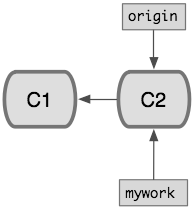
\includegraphics[width=0.20\textwidth]{content/git/rebase0.png}
\end{figure}

Now you do some work, creating two new commits.
\lstset{basicstyle=\scriptsize, numbers=none, captionpos=b, tabsize=4}
\begin{lstlisting}[caption=,language={bash},
breaklines=true,label=lst:]
$ vi file.txt
$ git commit
$ vi otherfile.txt
$ git commit
...
\end{lstlisting}

Meanwhile, someone else does some work creating two new commits on the origin
branch too. This means both 'origin' and 'mywork' has advanced, which means the
work has diverged.

\begin{figure}[h]
\centering
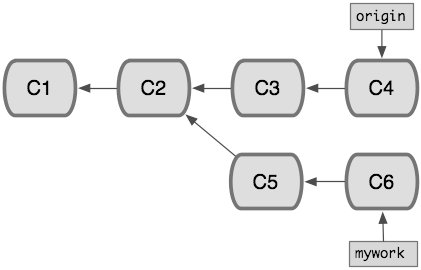
\includegraphics[width=0.43\textwidth]{content/git/rebase1.png}
\end{figure}

At this point, you could use "pull" to merge your changes back in; the result
would create a new merge commit, like this:

\begin{figure}[h]
\centering
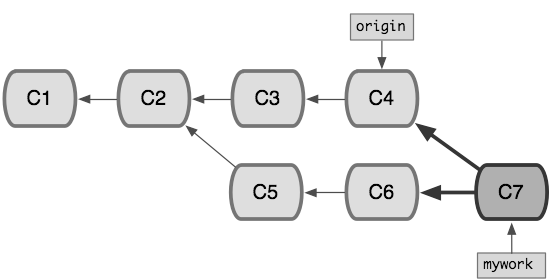
\includegraphics[width=0.43\textwidth]{content/git/rebase2.png}
\end{figure}

However, if you prefer to keep the history in mywork a simple series of commits
without any merges, you may instead choose to use git rebase:

\section{git merge}
\begin{figure}[h]
\centering
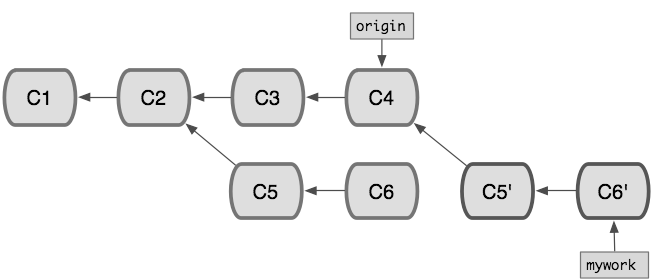
\includegraphics[width=0.43\textwidth]{content/git/rebase3.png}
\end{figure}

\lstset{basicstyle=\scriptsize, numbers=none, captionpos=b, tabsize=4}
\begin{lstlisting}[caption=,language={bash},
breaklines=true,label=lst:]
$ git checkout mywork
$ git rebase origin
\end{lstlisting}

This will remove each of your commits from mywork, temporarily saving them as
patches (in a directory named ".git/rebase"), update mywork to point at the
latest version of origin, then apply each of the saved patches to the new
mywork.

Once the ref ('mywork') is updated to point to the newly created commit
objects, your older commits will be abandoned. They will likely be removed if
you run a pruning garbage collection. (see git gc)
\begin{figure}[h]
\centering
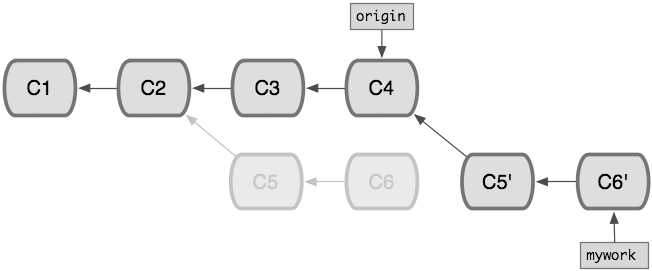
\includegraphics[width=0.43\textwidth]{content/git/rebase4.png}
\end{figure}

So now we can look at the difference in our history between running a merge and
running a rebase:
\begin{figure}[h]
\centering
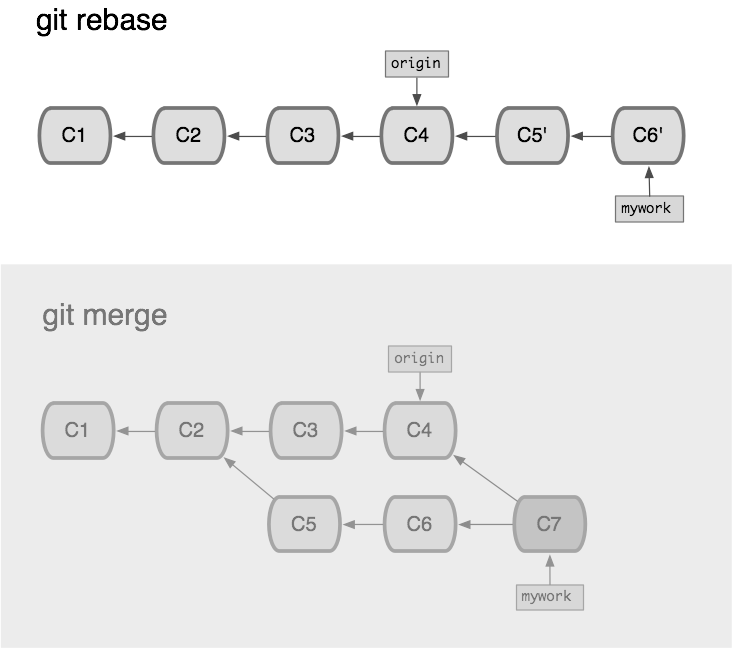
\includegraphics[width=0.43\textwidth]{content/git/rebase5.png}
\end{figure}


In the process of the rebase, it may discover conflicts. In that case it will
stop and allow you to fix the conflicts; after fixing conflicts, use "git-add"
to update the index with those contents, and then, instead of running
git-commit, just run
\lstset{basicstyle=\scriptsize, numbers=none, captionpos=b, tabsize=4}
\begin{lstlisting}[caption=,language={bash},
breaklines=true,label=lst:]
$ git rebase --continue
\end{lstlisting}

and git will continue applying the rest of the patches.

At any point you may use the --abort option to abort this process and return
mywork to the state it had before you started the rebase:

\lstset{basicstyle=\scriptsize, numbers=none, captionpos=b, tabsize=4}
\begin{lstlisting}[caption=,language={bash},
breaklines=true,label=lst:]
$ git rebase --abort
\end{lstlisting}

\subsection{Interactive Rebasing}
You can also rebase interactively. This is often used to re-write your own
commit objects before pusing them somewhere. It is an easy way to split, merge
or re-order commits before sharing them with others. You can also use it to
clean up commits you've pulled from someone when applying them locally.

If you have a number of commits that you would like to somehow modify during
the rebase, you can invoke interactive mode by passing a '-i' or
'--interactive' to the 'git rebase' command.
\lstset{basicstyle=\scriptsize, numbers=none, captionpos=b, tabsize=4}
\begin{lstlisting}[caption=,language={bash},
breaklines=true,label=lst:]
$ git rebase -i origin/master
\end{lstlisting}

This will invoke interactive rebase mode on all the commits you have made since
the last time you have pushed (or merged from the origin repository).

To see what commits those are beforehand, you can run log this way:

\lstset{basicstyle=\scriptsize, numbers=none, captionpos=b, tabsize=4}
\begin{lstlisting}[caption=,language={bash},
breaklines=true,label=lst:]
$ git log github/master..
\end{lstlisting}
Once you run the 'rebase -i' command, you will be thrown into your editor of
choice with something that looks like this:
\lstset{basicstyle=\scriptsize, numbers=none, captionpos=b, tabsize=4}
\begin{lstlisting}[caption=,language={bash},
breaklines=true,label=lst:]
pick fc62e55 added file_size
pick 9824bf4 fixed little thing
pick 21d80a5 added number to log
pick 76b9da6 added the apply command
pick c264051 Revert "added file_size" - not implemented correctly

# Rebase f408319..b04dc3d onto f408319
#
# Commands:
#  p, pick = use commit
#  e, edit = use commit, but stop for amending
#  s, squash = use commit, but meld into previous commit
#
# If you remove a line here THAT COMMIT WILL BE LOST.
# However, if you remove everything, the rebase will be aborted.
#
\end{lstlisting}

This means that there are 5 commits since you last pushed and it gives you one
line per commit with the following format:

(action) (partial-sha) (short commit message)
Now, you can change the action (which is by default 'pick') to either 'edit' or
'squash', or just leave it as 'pick'. You can also reorder the commits just by
moving the lines around however you want. Then, when you exit the editor, git
will try to apply the commits however they are now arranged and do the action
specified.

If 'pick' is specified, it will simply try to apply the patch and save the
commit with the same message as before.

If 'squash' is specified, it will combine that commit with the previous one to
create a new commit. This will drop you into your editor again to merge the
commit messages of the two commits it is now squashing together. So, if you
exit the editor with this:
\lstset{basicstyle=\scriptsize, numbers=none, captionpos=b, tabsize=4}
\begin{lstlisting}[caption=,language={bash},
breaklines=true,label=lst:]
pick   fc62e55 added file_size
squash 9824bf4 fixed little thing
squash 21d80a5 added number to log
squash 76b9da6 added the apply command
squash c264051 Revert "added file_size" - not implemented correctly
\end{lstlisting}

Then you will have to create a single commit message from this:
\lstset{basicstyle=\scriptsize, numbers=none, captionpos=b, tabsize=4}
\begin{lstlisting}[caption=,language={bash},
breaklines=true,label=lst:]
# This is a combination of 5 commits.
# The first commit's message is:
added file_size

# This is the 2nd commit message:

fixed little thing

# This is the 3rd commit message:

added number to log

# This is the 4th commit message:

added the apply command

# This is the 5th commit message:

Revert "added file_size" - not implemented correctly

This reverts commit
fc62e5543b195f18391886b9f663d5a7eca38e84.
\end{lstlisting}

Once you have edited that down into once commit message and exit the editor,
the commit will be saved with your new message.

If 'edit' is specified, it will do the same thing, but then pause before moving
on to the next one and drop you into the command line so you can amend the
commit, or change the commit contents somehow.

If you wanted to split a commit, for instance, you would specify 'edit' for
that commit:
\lstset{basicstyle=\scriptsize, numbers=none, captionpos=b, tabsize=4}
\begin{lstlisting}[caption=,language={bash},
breaklines=true,label=lst:]
pick   fc62e55 added file_size
pick   9824bf4 fixed little thing
edit   21d80a5 added number to log
pick   76b9da6 added the apply command
pick   c264051 Revert "added file_size" - not implemented correctly
\end{lstlisting}

And then when you get to the command line, you revert that commit and create
two (or more) new ones. Lets say 21d80a5 modified two files, file1 and file2,
and you wanted to split them into seperate commits. You could do this after the
rebase dropped you to the command line :
\lstset{basicstyle=\scriptsize, numbers=none, captionpos=b, tabsize=4}
\begin{lstlisting}[caption=,language={bash},
breaklines=true,label=lst:]
$ git reset HEAD^
$ git add file1
$ git commit 'first part of split commit'
$ git add file2
$ git commit 'second part of split commit'
$ git rebase --continue
\end{lstlisting}

And now instead of 5 commits, you would have 6.

The last useful thing that interactive rebase can do is drop commits for you.
If instead of choosing 'pick', 'squash' or 'edit' for the commit line, you
simply remove the line, it will remove the commit from the history.

\section{Interactive Adding}
Interactive Adding is a really nice way of working with and visualizing the Git
index. To start it up, simply type 'git add -i'. Git will show you all the
modified files you have and their status.
\lstset{basicstyle=\scriptsize, numbers=none, captionpos=b, tabsize=4}
\begin{lstlisting}[caption=,language={bash},
breaklines=true,label=lst:]
$>git add -i
           staged     unstaged path
  1:    unchanged        +4/-0 assets/stylesheets/style.css
  2:    unchanged      +23/-11 layout/book_index_template.html
  3:    unchanged        +7/-7 layout/chapter_template.html
  4:    unchanged        +3/-3 script/pdf.rb
  5:    unchanged      +121/-0 text/14_Interactive_Rebasing/0_ Interactive_Rebasing.markdown

*** Commands ***
  1: status   2: update   3: revert   4: add untracked
  5: patch    6: diff     7: quit     8: help
What now> 
\end{lstlisting}

In this case, we can see that there are 5 modified files that have not been
added to our index yet (unstaged), and even how many lines have been added to
or removed from each. It then shows us an interactive menu of what we can do in
this mode.

If we want to stage the files, we can type '2' or 'u' for the update mode. Then
I can specify which files I want to stage (add to the index) by typing in the
numbers of the files (in this case, 1-4)
\lstset{basicstyle=\scriptsize, numbers=none, captionpos=b, tabsize=4}
\begin{lstlisting}[caption=,language={bash},
breaklines=true,label=lst:]
What now> 2
           staged     unstaged path
  1:    unchanged        +4/-0 assets/stylesheets/style.css
  2:    unchanged      +23/-11 layout/book_index_template.html
  3:    unchanged        +7/-7 layout/chapter_template.html
  4:    unchanged        +3/-3 script/pdf.rb
  5:    unchanged      +121/-0 text/14_Interactive_Rebasing/0_ Interactive_Rebasing.markdown
Update>> 1-4
           staged     unstaged path
* 1:    unchanged        +4/-0 assets/stylesheets/style.css
* 2:    unchanged      +23/-11 layout/book_index_template.html
* 3:    unchanged        +7/-7 layout/chapter_template.html
* 4:    unchanged        +3/-3 script/pdf.rb
  5:    unchanged      +121/-0 text/14_Interactive_Rebasing/0_ Interactive_Rebasing.markdown
Update>> 
\end{lstlisting}

If I hit enter, I will be taken back to the main menu where I can see that the file status has changed:
\lstset{basicstyle=\scriptsize, numbers=none, captionpos=b, tabsize=4}
\begin{lstlisting}[caption=,language={bash},
breaklines=true,label=lst:]
What now> status
           staged     unstaged path
  1:        +4/-0      nothing assets/stylesheets/style.css
  2:      +23/-11      nothing layout/book_index_template.html
  3:        +7/-7      nothing layout/chapter_template.html
  4:        +3/-3      nothing script/pdf.rb
  5:    unchanged      +121/-0 text/14_Interactive_Rebasing/0_ Interactive_Rebasing.markdown
\end{lstlisting}

Now we can see the first four files are staged and the last one is still not.
This is basically a compressed way to see the same information we see when we
run 'git status' from the command line:
\lstset{basicstyle=\scriptsize, numbers=none, captionpos=b, tabsize=4}
\begin{lstlisting}[caption=,language={bash},
breaklines=true,label=lst:]
$ git status
# On branch master
# Changes to be committed:
#   (use "git reset HEAD <file>..." to unstage)
#
#   modified:   assets/stylesheets/style.css
#   modified:   layout/book_index_template.html
#   modified:   layout/chapter_template.html
#   modified:   script/pdf.rb
#
# Changed but not updated:
#   (use "git add <file>..." to update what will be committed)
#
#   modified:   text/14_Interactive_Rebasing/0_ Interactive_Rebasing.markdown
#
\end{lstlisting}

There are a number of useful things we can do, including unstaging files (3:
revert), adding untracked files (4: add untracked), and viewing diffs (6:
diff). Those are all pretty straightforward. However, there is one command that
is pretty cool here, which is staging patches (5: patch).

If you type '5' or 'p' in the menu, git will show you your diff patch by patch
(or hunk by hunk) and ask if you want to stage each one. That way you can
actually stage for a commit a part of a file edit. If you've edited a file and
want to only commit part of it and not an unfinished part, or commit
documentation or whitespace changes seperate from substantive changes, you can
use 'git add -i' to do so relatively easily.

Here I've staged some changes to the book\_index\_template.html file, but not all
of them:
\lstset{basicstyle=\scriptsize, numbers=none, captionpos=b, tabsize=4}
\begin{lstlisting}[caption=,language={bash},
breaklines=true,label=lst:]
         staged     unstaged path
1:        +4/-0      nothing assets/stylesheets/style.css
2:       +20/-7        +3/-4 layout/book_index_template.html
3:        +7/-7      nothing layout/chapter_template.html
4:        +3/-3      nothing script/pdf.rb
5:    unchanged      +121/-0 text/14_Interactive_Rebasing/0_ Interactive_Rebasing.markdown
6:    unchanged       +85/-0 text/15_Interactive_Adding/0_ Interactive_Adding.markdown
\end{lstlisting}

When you are done making changes to your index through 'git add -i', you simply
quit (7: quit) and then run 'git commit' to commit the staged changes. Remember
not to run 'git commit -a', which will blow away all the careful changes you've
just made and simply commit everything.

\subsection{Stashing}
While you are in the middle of working on something complicated, you find an
unrelated but obvious and trivial bug. You would like to fix it before
continuing. You can use git stash to save the current state of your work, and
after fixing the bug (or, optionally after doing so on a different branch and
then coming back), unstash the work-in-progress changes.
\lstset{basicstyle=\scriptsize, numbers=none, captionpos=b, tabsize=4}
\begin{lstlisting}[caption=,language={bash},
breaklines=true,label=lst:]
$ git stash "work in progress for foo feature"
\end{lstlisting}

This command will save your changes away to the stash, and reset your working
tree and the index to match the tip of your current branch. Then you can make
your fix as usual.
\lstset{basicstyle=\scriptsize, numbers=none, captionpos=b, tabsize=4}
\begin{lstlisting}[caption=,language={bash},
breaklines=true,label=lst:]
... edit and test ...
$ git commit -a -m "blorpl: typofix"
\end{lstlisting}

After that, you can go back to what you were working on with git stash apply:
\lstset{basicstyle=\scriptsize, numbers=none, captionpos=b, tabsize=4}
\begin{lstlisting}[caption=,language={bash},
breaklines=true,label=lst:]
$ git stash apply
\end{lstlisting}

\subsubsection{Stash Queue}
You can also use stashing to queue up stashed changes.  If you run 'git stash
list' you can see which stashes you have saved:
\lstset{basicstyle=\scriptsize, numbers=none, captionpos=b, tabsize=4}
\begin{lstlisting}[caption=,language={bash},
breaklines=true,label=lst:]
$>git stash list
stash@{0}: WIP on book: 51bea1d... fixed images
stash@{1}: WIP on master: 9705ae6... changed the browse code to the official repo
\end{lstlisting}

Then you can apply them individually with 'git stash apply stash@{1}'. You can
clear out the list with 'git stash clear'.

\subsection{Git Treeishes}
There are a number of ways to refer to a particular commit or tree other than
spelling out the entire 40-character sha. In Git, these are referred to as a
'treeish'.

\subsubsection{Partial Sha}
If your commit sha is '980e3ccdaac54a0d4de358f3fe5d718027d96aae', git will
recognize any of the following identically:
\lstset{basicstyle=\scriptsize, numbers=none, captionpos=b, tabsize=4}
\begin{lstlisting}[caption=,language={bash},
breaklines=true,label=lst:]
980e3ccdaac54a0d4de358f3fe5d718027d96aae
980e3ccdaac54a0d4
980e3cc
\end{lstlisting}

As long as the partial sha is unique - it can't be confused with another (which
is incredibly unlikely if you use at least 5 characters), git will expand a
partial sha for you.

\subsubsection{Branch, Remote or Tag Name}
You can always use a branch, remote or tag name instead of a sha, since they
are simply pointers anyhow. If your master branch is on the 980e3 commit and
you've pushed it to origin and have tagged it 'v1.0', then all of the following
are equivalent:
\lstset{basicstyle=\scriptsize, numbers=none, captionpos=b, tabsize=4}
\begin{lstlisting}[caption=,language={bash},
breaklines=true,label=lst:]

980e3ccdaac54a0d4de358f3fe5d718027d96aae
origin/master
refs/remotes/origin/master
master
refs/heads/master
v1.0
refs/tags/v1.0
\end{lstlisting}

Which means the following will give you identical output:
\lstset{basicstyle=\scriptsize, numbers=none, captionpos=b, tabsize=4}
\begin{lstlisting}[caption=,language={bash},
breaklines=true,label=lst:]
$ git log master

$ git log refs/tags/v1.0
\end{lstlisting}

\subsubsection{Date Spec}
The Ref Log that git keeps will allow you to do some relative stuff locally,
such as:
\lstset{basicstyle=\scriptsize, numbers=none, captionpos=b, tabsize=4}
\begin{lstlisting}[caption=,language={bash},
breaklines=true,label=lst:]
master@{yesterday}

master@{1 month ago}
\end{lstlisting}

Which is shorthand for 'where the master branch head was yesterday', etc. Note
that this format can result in different shas on different computers, even if
the master branch is currently pointing to the same place.

\subsubsection{Ordinal Spec}
This format will give you the Nth previous value of a particular reference. For
example:
\lstset{basicstyle=\scriptsize, numbers=none, captionpos=b, tabsize=4}
\begin{lstlisting}[caption=,language={bash},
breaklines=true,label=lst:]
master@{5}
\end{lstlisting}

will give you the 5th prior value of the master head ref.

\subsubsection{Carrot Parent}
This will give you the Nth parent of a particular commit. This format is only
useful on merge commits - commit objects that have more than one direct parent.
\lstset{basicstyle=\scriptsize, numbers=none, captionpos=b, tabsize=4}
\begin{lstlisting}[caption=,language={bash},
breaklines=true,label=lst:]
master^2
\end{lstlisting}

\subsubsection{Tilde Spec}
The tilde spec will give you the Nth grandparent of a commit object. For
example,
\lstset{basicstyle=\scriptsize, numbers=none, captionpos=b, tabsize=4}
\begin{lstlisting}[caption=,language={bash},
breaklines=true,label=lst:]
master~2
\end{lstlisting}

will give us the first parent of the first parent of the commit that master
points to. It is equivalent to:
\lstset{basicstyle=\scriptsize, numbers=none, captionpos=b, tabsize=4}
\begin{lstlisting}[caption=,language={bash},
breaklines=true,label=lst:]
master^^
\end{lstlisting}

You can keep doing this, too. The following specs will point to the same
commit:
\lstset{basicstyle=\scriptsize, numbers=none, captionpos=b, tabsize=4}
\begin{lstlisting}[caption=,language={bash},
breaklines=true,label=lst:]
master^^^^^^
master~3^~2
master~6
\end{lstlisting}

\subsubsection{Tree Pointer}
This disambiguates a commit from the tree that it points to. If you want the
sha that a commit points to, you can add the '\^{tree}' spec to the end of it.
\lstset{basicstyle=\scriptsize, numbers=none, captionpos=b, tabsize=4}
\begin{lstlisting}[caption=,language={bash},
breaklines=true,label=lst:]
master^{tree}
\end{lstlisting}

\subsubsection{Blob Spec}
If you want the sha of a particular blob, you can add the blob path at the end
of the treeish, like so:
\lstset{basicstyle=\scriptsize, numbers=none, captionpos=b, tabsize=4}
\begin{lstlisting}[caption=,language={bash},
breaklines=true,label=lst:]
master:/path/to/file
\end{lstlisting}

\subsubsection{Range}
Finally, you can specify a range of commits with the range spec. This will give
you all the commits between 7b593b5 and 51bea1 (where 51bea1 is most recent),
excluding 7b593b5 but including 51bea1:
\lstset{basicstyle=\scriptsize, numbers=none, captionpos=b, tabsize=4}
\begin{lstlisting}[caption=,language={bash},
breaklines=true,label=lst:]
7b593b5..51bea1
\end{lstlisting}

This will include every commit since 7b593b:
\lstset{basicstyle=\scriptsize, numbers=none, captionpos=b, tabsize=4}
\begin{lstlisting}[caption=,language={bash},
breaklines=true,label=lst:]
7b593b.. 
\end{lstlisting}

\section{Tracking Branches}
A 'tracking branch' in Git is a local branch that is connected to a remote
branch. When you push and pull on that branch, it automatically pushes and
pulls to the remote branch that it is connected with.

Use this if you always pull from the same upstream branch into the new branch,
and if you don't want to use "git pull " explicitly.

The 'git clone' command automatically sets up a 'master' branch that is a
tracking branch for 'origin/master' - the master branch on the cloned
repository.

You can create a tracking branch manually by adding the '--track' option to the
'branch' command in Git.
\lstset{basicstyle=\scriptsize, numbers=none, captionpos=b, tabsize=4}
\begin{lstlisting}[caption=,language={bash},
breaklines=true,label=lst:]
git branch --track experimental origin/experimental
\end{lstlisting}

Then when you run:
\lstset{basicstyle=\scriptsize, numbers=none, captionpos=b, tabsize=4}
\begin{lstlisting}[caption=,language={bash},
breaklines=true,label=lst:]
$ git pull experimental
\end{lstlisting}

It will automatically fetch from 'origin' and merge 'origin/experimental' into
your local 'experimental' branch.

Likewise, when you push to origin, it will push what your 'experimental' points
to to origins 'experimental', without having to specify it.

\subsection{Finding with Git Grep}
Finding files with words or phrases in Git is really easy with the git grep
command. It is possible to do this with the normal unix 'grep' command, but
with 'git grep' you can also search through previous versions of the project
without having to check them out.

For example, if I wanted to see every place that used the 'xmmap' call in my
git.git repository, I could run this:
\lstset{basicstyle=\scriptsize, numbers=none, captionpos=b, tabsize=4}
\begin{lstlisting}[caption=,language={bash},
breaklines=true,label=lst:]
$ git grep xmmap
config.c:               contents = xmmap(NULL, contents_sz, PROT_READ,
diff.c:         s->data = xmmap(NULL, s->size, PROT_READ, MAP_PRIVATE, fd, 0);
git-compat-util.h:extern void *xmmap(void *start, size_t length, int prot, int fla
read-cache.c:   mmap = xmmap(NULL, mmap_size, PROT_READ | PROT_WRITE, MAP_PRIVATE,
refs.c: log_mapped = xmmap(NULL, mapsz, PROT_READ, MAP_PRIVATE, logfd, 0);
sha1_file.c:    map = xmmap(NULL, mapsz, PROT_READ, MAP_PRIVATE, fd, 0);
sha1_file.c:    idx_map = xmmap(NULL, idx_size, PROT_READ, MAP_PRIVATE, fd, 0);
sha1_file.c:                    win->base = xmmap(NULL, win->len,
sha1_file.c:                    map = xmmap(NULL, *size, PROT_READ, MAP_PRIVATE, f
sha1_file.c:            buf = xmmap(NULL, size, PROT_READ, MAP_PRIVATE, fd, 0);
wrapper.c:void *xmmap(void *start, size_t length,
\end{lstlisting}

If I wanted to see the line number of each match as well, I can add the '-n'
option:
\lstset{basicstyle=\scriptsize, numbers=none, captionpos=b, tabsize=4}
\begin{lstlisting}[caption=,language={bash},
breaklines=true,label=lst:]
$>git grep -n xmmap
config.c:1016:          contents = xmmap(NULL, contents_sz, PROT_READ,
diff.c:1833:            s->data = xmmap(NULL, s->size, PROT_READ, MAP_PRIVATE, fd,
git-compat-util.h:291:extern void *xmmap(void *start, size_t length, int prot, int
read-cache.c:1178:      mmap = xmmap(NULL, mmap_size, PROT_READ | PROT_WRITE, MAP_
refs.c:1345:    log_mapped = xmmap(NULL, mapsz, PROT_READ, MAP_PRIVATE, logfd, 0);
sha1_file.c:377:        map = xmmap(NULL, mapsz, PROT_READ, MAP_PRIVATE, fd, 0);
sha1_file.c:479:        idx_map = xmmap(NULL, idx_size, PROT_READ, MAP_PRIVATE, fd
sha1_file.c:780:                        win->base = xmmap(NULL, win->len,
sha1_file.c:1076:                       map = xmmap(NULL, *size, PROT_READ, MAP_PR
sha1_file.c:2393:               buf = xmmap(NULL, size, PROT_READ, MAP_PRIVATE, fd
wrapper.c:89:void *xmmap(void *start, size_t length,
\end{lstlisting}

If we're only interested in the filename, we can pass the '--name-only' option:
\lstset{basicstyle=\scriptsize, numbers=none, captionpos=b, tabsize=4}
\begin{lstlisting}[caption=,language={bash},
breaklines=true,label=lst:]
$>git grep --name-only xmmap
config.c
diff.c
git-compat-util.h
read-cache.c
refs.c
sha1_file.c
wrapper.c
\end{lstlisting}

We could also see how many line matches we have in each file with the '-c'
option:
\lstset{basicstyle=\scriptsize, numbers=none, captionpos=b, tabsize=4}
\begin{lstlisting}[caption=,language={bash},
breaklines=true,label=lst:]
$>git grep -c xmmap
config.c:1
diff.c:1
git-compat-util.h:1
read-cache.c:1
refs.c:1
sha1_file.c:5
wrapper.c:1
\end{lstlisting}

Now, if I wanted to see where that was used in a specific version of git, I
could add the tag reference to the end, like this:
\lstset{basicstyle=\scriptsize, numbers=none, captionpos=b, tabsize=4}
\begin{lstlisting}[caption=,language={bash},
breaklines=true,label=lst:]
$ git grep xmmap v1.5.0
v1.5.0:config.c:                contents = xmmap(NULL, st.st_size, PROT_READ,
v1.5.0:diff.c:          s->data = xmmap(NULL, s->size, PROT_READ, MAP_PRIVATE, fd,
v1.5.0:git-compat-util.h:static inline void *xmmap(void *start, size_t length,
v1.5.0:read-cache.c:                    cache_mmap = xmmap(NULL, cache_mmap_size, 
v1.5.0:refs.c:  log_mapped = xmmap(NULL, st.st_size, PROT_READ, MAP_PRIVATE, logfd
v1.5.0:sha1_file.c:     map = xmmap(NULL, st.st_size, PROT_READ, MAP_PRIVATE, fd, 
v1.5.0:sha1_file.c:     idx_map = xmmap(NULL, idx_size, PROT_READ, MAP_PRIVATE, fd
v1.5.0:sha1_file.c:                     win->base = xmmap(NULL, win->len,
v1.5.0:sha1_file.c:     map = xmmap(NULL, st.st_size, PROT_READ, MAP_PRIVATE, fd, 
v1.5.0:sha1_file.c:             buf = xmmap(NULL, size, PROT_READ, MAP_PRIVATE, fd
\end{lstlisting}

We can see that there are some differences between the current lines and these
lines in version 1.5.0, one of which is that xmmap is now used in wrapper.c
where it was not back in v1.5.0.

We can also combine search terms in grep. Say we wanted to search for where
SORT\_DIRENT is defined in our repository:
\lstset{basicstyle=\scriptsize, numbers=none, captionpos=b, tabsize=4}
\begin{lstlisting}[caption=,language={bash},
breaklines=true,label=lst:]
$ git grep -e '#define' --and -e SORT_DIRENT
builtin-fsck.c:#define SORT_DIRENT 0
builtin-fsck.c:#define SORT_DIRENT 1
\end{lstlisting}

We can also search for every file that has both search terms, but display each
line that has either of the terms in those files:
\lstset{basicstyle=\scriptsize, numbers=none, captionpos=b, tabsize=4}
\begin{lstlisting}[caption=,language={bash},
breaklines=true,label=lst:]
$ git grep --all-match -e '#define' -e SORT_DIRENT
builtin-fsck.c:#define REACHABLE 0x0001
builtin-fsck.c:#define SEEN      0x0002
builtin-fsck.c:#define ERROR_OBJECT 01
builtin-fsck.c:#define ERROR_REACHABLE 02
builtin-fsck.c:#define SORT_DIRENT 0
builtin-fsck.c:#define DIRENT_SORT_HINT(de) 0
builtin-fsck.c:#define SORT_DIRENT 1
builtin-fsck.c:#define DIRENT_SORT_HINT(de) ((de)->d_ino)
builtin-fsck.c:#define MAX_SHA1_ENTRIES (1024)
builtin-fsck.c: if (SORT_DIRENT)
\end{lstlisting}

We can also search for lines that have one term and either of two other terms,
for example, if we wanted to see where we defined constants that had either
PATH or MAX in the name:
\lstset{basicstyle=\scriptsize, numbers=none, captionpos=b, tabsize=4}
\begin{lstlisting}[caption=,language={bash},
breaklines=true,label=lst:]
$ git grep -e '#define' --and \( -e PATH -e MAX \) 
abspath.c:#define MAXDEPTH 5
builtin-blame.c:#define MORE_THAN_ONE_PATH      (1u<<13)
builtin-blame.c:#define MAXSG 16
builtin-describe.c:#define MAX_TAGS     (FLAG_BITS - 1)
builtin-fetch-pack.c:#define MAX_IN_VAIN 256
builtin-fsck.c:#define MAX_SHA1_ENTRIES (1024)
...
\end{lstlisting}

\section{Undoing in Git - Reset, Checkout and Revert}
Git provides multiple methods for fixing up mistakes as you are developing.
Selecting an appropriate method depends on whether or not you have committed
the mistake, and if you have committed the mistake, whether you have shared the
erroneous commit with anyone else.

\subsection{Fixing un-committed mistakes}
If you've messed up the working tree, but haven't yet committed your mistake,
you can return the entire working tree to the last committed state with
\lstset{basicstyle=\scriptsize, numbers=none, captionpos=b, tabsize=4}
\begin{lstlisting}[caption=,language={bash},
breaklines=true,label=lst:]
$ git reset --hard HEAD
\end{lstlisting}

This will throw away any changes you may have added to the git index and as
well as any outstanding changes you have in your working tree. In other words,
it causes the results of "git diff" and "git diff --cached" to both be empty.

If you just want to restore just one file, say your hello.rb, use git checkout
instead
\lstset{basicstyle=\scriptsize, numbers=none, captionpos=b, tabsize=4}
\begin{lstlisting}[caption=,language={bash},
breaklines=true,label=lst:]
$ git checkout -- hello.rb
$ git checkout HEAD hello.rb
\end{lstlisting}

The first command restores hello.rb to the version in the index, so that "git
diff hello.rb" returns no differences. The second command will restore hello.rb
to the version in the HEAD revision, so that both "git diff hello.rb" and "git
diff --cached hello.rb" return no differences.

\subsection{Fixing committed mistakes}
If you make a commit that you later wish you hadn't, there are two
fundamentally different ways to fix the problem:
\begin{enumerate}
\item You can create a new commit that undoes whatever was done by the old commit.
This is the correct thing if your mistake has already been made public.

\item You can go back and modify the old commit. You should never do this if you have
already made the history public; git does not normally expect the "history" of
a project to change, and cannot correctly perform repeated merges from a branch
that has had its history changed.
\end{enumerate}

\subsection{Fixing a mistake with a new commit}
Creating a new commit that reverts an earlier change is very easy; just pass
the git revert command a reference to the bad commit; for example, to revert
the most recent commit:
\lstset{basicstyle=\scriptsize, numbers=none, captionpos=b, tabsize=4}
\begin{lstlisting}[caption=,language={bash},
breaklines=true,label=lst:]
$ git revert HEAD
\end{lstlisting}

This will create a new commit which undoes the change in HEAD. You will be
given a chance to edit the commit message for the new commit.

You can also revert an earlier change, for example, the next-to-last:
\lstset{basicstyle=\scriptsize, numbers=none, captionpos=b, tabsize=4}
\begin{lstlisting}[caption=,language={bash},
breaklines=true,label=lst:]
$ git revert HEAD^
\end{lstlisting}

In this case git will attempt to undo the old change while leaving intact any
changes made since then. If more recent changes overlap with the changes to be
reverted, then you will be asked to fix conflicts manually, just as in the case
of resolving a merge.

\subsection{Fixing a mistake by modifying a commit}
If you have just committed something but realize you need to fix up that
commit, recent versions of git commit support an --amend flag which instructs
git to replace the HEAD commit with a new one, based on the current contents of
the index. This gives you an opportunity to add files that you forgot to add or
correct typos in a commit message, prior to pushing the change out for the
world to see.

If you find a mistake in an older commit, but still one that you have not yet
published to the world, you use git rebase in interactive mode, with "git
rebase -i" marking the change that requires correction with edit. This will
allow you to amend the commit during the rebasing process.

\subsection{Maintaining Git}
Ensuring good performance

On large repositories, git depends on compression to keep the history
information from taking up too much space on disk or in memory.

This compression is not performed automatically. Therefore you should
occasionally run git gc:
\lstset{basicstyle=\scriptsize, numbers=none, captionpos=b, tabsize=4}
\begin{lstlisting}[caption=,language={bash},
breaklines=true,label=lst:]
$ git gc
\end{lstlisting}

to recompress the archive. This can be very time-consuming, so you may prefer
to run git-gc when you are not doing other work.

\subsubsection{Ensuring reliability}
The git fsck command runs a number of self-consistency checks on the
repository, and reports on any problems. This may take some time. The most
common warning by far is about "dangling" objects:
\lstset{basicstyle=\scriptsize, numbers=none, captionpos=b, tabsize=4}
\begin{lstlisting}[caption=,language={bash},
breaklines=true,label=lst:]
$ git fsck
dangling commit 7281251ddd2a61e38657c...
dangling commit 2706a059f258c6b245f29...
dangling commit 13472b7c4b80851a1bc55...
dangling blob 218761f9d90712d37a9c5e3...
dangling commit bf093535a34a4d35731aa...
dangling commit 8e4bec7f2ddaa268bef99...
dangling tree d50bb86186bf27b681d25af...
dangling tree b24c2473f1fd3d91352a624...
...
\end{lstlisting}

Dangling objects are not a problem. At worst they may take up a little extra
disk space. They can sometimes provide a last-resort method for recovering lost
work.

\subsection{Setting Up A Public Repository}
Assume your personal repository is in the directory ~/proj. We first create a
new clone of the repository and tell git-daemon that it is meant to be public:
\lstset{basicstyle=\scriptsize, numbers=none, captionpos=b, tabsize=4}
\begin{lstlisting}[caption=,language={bash},
breaklines=true,label=lst:]
$ git clone --bare ~/proj proj.git
$ touch proj.git/git-daemon-export-ok
\end{lstlisting}

The resulting directory proj.git contains a "bare" git repository--it is just
the contents of the ".git" directory, without any files checked out around it.

Next, copy proj.git to the server where you plan to host the public repository.
You can use scp, rsync, or whatever is most convenient.

\subsubsection{Exporting a git repository via the git protocol}
This is the preferred method.

If someone else administers the server, they should tell you what directory to
put the repository in, and what git:// URL it will appear at.

Otherwise, all you need to do is start git daemon; it will listen on port 9418.
By default, it will allow access to any directory that looks like a git
directory and contains the magic file git-daemon-export-ok. Passing some
directory paths as git-daemon arguments will further restrict the exports to
those paths.

You can also run git-daemon as an inetd service; see the git daemon man page
for details. (See especially the examples section.)

\subsubsection{Exporting a git repository via http}
The git protocol gives better performance and reliability, but on a host with a
web server set up, http exports may be simpler to set up.

All you need to do is place the newly created bare git repository in a
directory that is exported by the web server, and make some adjustments to give
web clients some extra information they need:
\lstset{basicstyle=\scriptsize, numbers=none, captionpos=b, tabsize=4}
\begin{lstlisting}[caption=,language={bash},
breaklines=true,label=lst:]
$ mv proj.git /home/you/public_html/proj.git
$ cd proj.git
$ git --bare update-server-info
$ chmod a+x hooks/post-update
\end{lstlisting}

(For an explanation of the last two lines, see git update-server-info and
githooks.)

Advertise the URL of proj.git. Anybody else should then be able to clone or
pull from that URL, for example with a command line like:
\lstset{basicstyle=\scriptsize, numbers=none, captionpos=b, tabsize=4}
\begin{lstlisting}[caption=,language={bash},
breaklines=true,label=lst:]
$ git clone http://yourserver.com/~you/proj.git
\end{lstlisting}

\subsection{Setting Up a Private Repository}
If you need to setup a private repository and want to do so locally, rather
than using a hosted solution, you have a number of options.

\subsubsection{Repo Access over SSH}
Generally, the easiest solution is to simply use Git over SSH. If users already
have ssh accounts on a machine, you can put the git repository anywhere on the
box that they have access to and let them access it over normal ssh logins. For
example, say you have a repository you want to host. You can export it as a
bare repo and then scp it onto your server like so:
\lstset{basicstyle=\scriptsize, numbers=none, captionpos=b, tabsize=4}
\begin{lstlisting}[caption=,language={bash},
breaklines=true,label=lst:]
$ git clone --bare /home/user/myrepo/.git /tmp/myrepo.git
$ scp -r /tmp/myrepo.git myserver.com:/opt/git/myrepo.git
\end{lstlisting}

Then someone else with an ssh account on myserver.com can clone via:
\lstset{basicstyle=\scriptsize, numbers=none, captionpos=b, tabsize=4}
\begin{lstlisting}[caption=,language={bash},
breaklines=true,label=lst:]
$ git clone myserver.com:/opt/git/myrepo.git
\end{lstlisting}

Which will simply prompt them for thier ssh password or use thier public key,
however they have ssh authentication setup.

\section{Advanced Git}
\section{Advanced Branching And Merging}
\subsection{Getting conflict-resolution help during a merge}

All of the changes that git was able to merge automatically are already added
to the index file, so git diff shows only the conflicts. It uses an unusual
syntax:
\lstset{basicstyle=\scriptsize, numbers=none, captionpos=b, tabsize=4}
\begin{lstlisting}[caption=,language={bash},
breaklines=true,label=lst:]
$ git diff
diff --cc file.txt
index 802992c,2b60207..0000000
--- a/file.txt
+++ b/file.txt
@@@ -1,1 -1,1 +1,5 @@@
++<<<<<<< HEAD:file.txt
 +Hello world
++=======
+ Goodbye
++>>>>>>> 77976da35a11db4580b80ae27e8d65caf5208086:file.txt
\end{lstlisting}

Recall that the commit which will be committed after we resolve this conflict
will have two parents instead of the usual one: one parent will be HEAD, the
tip of the current branch; the other will be the tip of the other branch, which
is stored temporarily in MERGE\_HEAD.

During the merge, the index holds three versions of each file. Each of these
three "file stages" represents a different version of the file:
\lstset{basicstyle=\scriptsize, numbers=none, captionpos=b, tabsize=4}
\begin{lstlisting}[caption=,language={bash},
breaklines=true,label=lst:]
$ git show :1:file.txt  # the file in a common ancestor of both branches
$ git show :2:file.txt  # the version from HEAD.
$ git show :3:file.txt  # the version from MERGE_HEAD.
\end{lstlisting}

When you ask git diff to show the conflicts, it runs a three-way diff between
the conflicted merge results in the work tree with stages 2 and 3 to show only
hunks whose contents come from both sides, mixed (in other words, when a hunk's
merge results come only from stage 2, that part is not conflicting and is not
shown. Same for stage 3).

The diff above shows the differences between the working-tree version of
file.txt and the stage 2 and stage 3 versions. So instead of preceding each
line by a single "+" or "-", it now uses two columns: the first column is used
for differences between the first parent and the working directory copy, and
the second for differences between the second parent and the working directory
copy. (See the "COMBINED DIFF FORMAT" section of git diff-files for a details
of the format.)

After resolving the conflict in the obvious way (but before updating the
index), the diff will look like:
\lstset{basicstyle=\scriptsize, numbers=none, captionpos=b, tabsize=4}
\begin{lstlisting}[caption=,language={bash},
breaklines=true,label=lst:]
$ git diff
diff --cc file.txt
index 802992c,2b60207..0000000
--- a/file.txt
+++ b/file.txt
@@@ -1,1 -1,1 +1,1 @@@
- Hello world
-Goodbye
++Goodbye world
\end{lstlisting}

This shows that our resolved version deleted "Hello world" from the first
parent, deleted "Goodbye" from the second parent, and added "Goodbye world",
which was previously absent from both.

Some special diff options allow diffing the working directory against any of
these stages:
\lstset{basicstyle=\scriptsize, numbers=none, captionpos=b, tabsize=4}
\begin{lstlisting}[caption=,language={bash},
breaklines=true,label=lst:]
$ git diff -1 file.txt      # diff against stage 1
$ git diff --base file.txt  # same as the above
$ git diff -2 file.txt      # diff against stage 2
$ git diff --ours file.txt  # same as the above
$ git diff -3 file.txt      # diff against stage 3
$ git diff --theirs file.txt    # same as the above.
\end{lstlisting}

The git log and gitk commands also provide special help for merges:
\lstset{basicstyle=\scriptsize, numbers=none, captionpos=b, tabsize=4}
\begin{lstlisting}[caption=,language={bash},
breaklines=true,label=lst:]
$ git log --merge
$ gitk --merge
\end{lstlisting}

These will display all commits which exist only on HEAD or on MERGE\_HEAD, and
which touch an unmerged file.

You may also use git mergetool, which lets you merge the unmerged files using
external tools such as emacs or kdiff3.

Each time you resolve the conflicts in a file and update the index:
\lstset{basicstyle=\scriptsize, numbers=none, captionpos=b, tabsize=4}
\begin{lstlisting}[caption=,language={bash},
breaklines=true,label=lst:]
$ git add file.txt
\end{lstlisting}

the different stages of that file will be "collapsed", after which git-diff
will (by default) no longer show diffs for that file.

\subsection{Multiway Merge}
You can merge several heads at one time by simply listing them on the same git
merge command. For instance,
\lstset{basicstyle=\scriptsize, numbers=none, captionpos=b, tabsize=4}
\begin{lstlisting}[caption=,language={bash},
breaklines=true,label=lst:]
$ git merge scott/master rick/master tom/master
\end{lstlisting}

is the equivalent of:
\lstset{basicstyle=\scriptsize, numbers=none, captionpos=b, tabsize=4}
\begin{lstlisting}[caption=,language={bash},
breaklines=true,label=lst:]
$ git merge scott/master
$ git merge rick/master
$ git merge tom/master
\end{lstlisting}

\subsection{Subtree}
There are situations where you want to include contents in your project from an
independently developed project. You can just pull from the other project as
long as there are no conflicting paths.

The problematic case is when there are conflicting files. Potential candidates
are Makefiles and other standard filenames. You could merge these files but
probably you do not want to. A better solution for this problem can be to merge
the project as its own subdirectory. This is not supported by the recursive
merge strategy, so just pulling won't work.

What you want is the subtree merge strategy, which helps you in such a
situation.

In this example, let's say you have the repository at /path/to/B (but it can be
an URL as well, if you want). You want to merge the master branch of that
repository to the dir-B subdirectory in your current branch.

Here is the command sequence you need:
\lstset{basicstyle=\scriptsize, numbers=none, captionpos=b, tabsize=4}
\begin{lstlisting}[caption=,language={bash},
breaklines=true,label=lst:]
$ git remote add -f Bproject /path/to/B (1)
$ git merge -s ours --no-commit Bproject/master (2)
$ git read-tree --prefix=dir-B/ -u Bproject/master (3)
$ git commit -m "Merge B project as our subdirectory" (4)
$ git pull -s subtree Bproject master (5)
\end{lstlisting}

The benefit of using subtree merge is that it requires less administrative
burden from the users of your repository. It works with older (before Git
v1.5.2) clients and you have the code right after clone.

However if you use submodules then you can choose not to transfer the submodule
objects. This may be a problem with the subtree merge.

Also, in case you make changes to the other project, it is easier to submit
changes if you just use submodules.

\section{Finding Issues - Git Bisect}
Suppose version 2.6.18 of your project worked, but the version at "master"
crashes. Sometimes the best way to find the cause of such a regression is to
perform a brute-force search through the project's history to find the
particular commit that caused the problem. The git bisect command can help you
do this:
\lstset{basicstyle=\scriptsize, numbers=none, captionpos=b, tabsize=4}
\begin{lstlisting}[caption=,language={bash},
breaklines=true,label=lst:]
$ git bisect start
$ git bisect good v2.6.18
$ git bisect bad master
Bisecting: 3537 revisions left to test after this
[65934a9a028b88e83e2b0f8b36618fe503349f8e] BLOCK: Make USB storage depend on SCSI rather than selecting it [try #6]
\end{lstlisting}

If you run "git branch" at this point, you'll see that git has temporarily
moved you to a new branch named "bisect". This branch points to a commit (with
commit id 65934...) that is reachable from "master" but not from v2.6.18.
Compile and test it, and see whether it crashes. Assume it does crash. Then:
\lstset{basicstyle=\scriptsize, numbers=none, captionpos=b, tabsize=4}
\begin{lstlisting}[caption=,language={bash},
breaklines=true,label=lst:]
$ git bisect bad
Bisecting: 1769 revisions left to test after this
[7eff82c8b1511017ae605f0c99ac275a7e21b867] i2c-core: Drop useless bitmaskings
\end{lstlisting}

checks out an older version. Continue like this, telling git at each stage
whether the version it gives you is good or bad, and notice that the number of
revisions left to test is cut approximately in half each time.

After about 13 tests (in this case), it will output the commit id of the guilty
commit. You can then examine the commit with git show, find out who wrote it,
and mail them your bug report with the commit id. Finally, run
\lstset{basicstyle=\scriptsize, numbers=none, captionpos=b, tabsize=4}
\begin{lstlisting}[caption=,language={bash},
breaklines=true,label=lst:]
$ git bisect reset
\end{lstlisting}

to return you to the branch you were on before and delete the temporary
"bisect" branch.

Note that the version which git-bisect checks out for you at each point is just
a suggestion, and you're free to try a different version if you think it would
be a good idea. For example, occasionally you may land on a commit that broke
something unrelated; run
\lstset{basicstyle=\scriptsize, numbers=none, captionpos=b, tabsize=4}
\begin{lstlisting}[caption=,language={bash},
breaklines=true,label=lst:]
$ git bisect visualize
\end{lstlisting}

which will run gitk and label the commit it chose with a marker that says
"bisect". Choose a safe-looking commit nearby, note its commit id, and check it
out with:
\lstset{basicstyle=\scriptsize, numbers=none, captionpos=b, tabsize=4}
\begin{lstlisting}[caption=,language={bash},
breaklines=true,label=lst:]
$ git reset --hard fb47ddb2db...
\end{lstlisting}

then test, run "bisect good" or "bisect bad" as appropriate, and continue.

\subsection{Finding Issues - Git Blame}
The git blame command is really helpful for figuring out who changed which
sections of a file. If you simple run 'git blame [filename]' you'll get an
output of the entire file with the last commit sha, date and author for every
line in the file.
\lstset{basicstyle=\scriptsize, numbers=none, captionpos=b, tabsize=4}
\begin{lstlisting}[caption=,language={bash},
breaklines=true,label=lst:]
$ git blame sha1_file.c
...
0fcfd160 (Linus Torvalds  2005-04-18 13:04:43 -0700    8)  */
0fcfd160 (Linus Torvalds  2005-04-18 13:04:43 -0700    9) #include "cache.h"
1f688557 (Junio C Hamano  2005-06-27 03:35:33 -0700   10) #include "delta.h"
a733cb60 (Linus Torvalds  2005-06-28 14:21:02 -0700   11) #include "pack.h"
8e440259 (Peter Eriksen   2006-04-02 14:44:09 +0200   12) #include "blob.h"
8e440259 (Peter Eriksen   2006-04-02 14:44:09 +0200   13) #include "commit.h"
8e440259 (Peter Eriksen   2006-04-02 14:44:09 +0200   14) #include "tag.h"
8e440259 (Peter Eriksen   2006-04-02 14:44:09 +0200   15) #include "tree.h"
f35a6d3b (Linus Torvalds  2007-04-09 21:20:29 -0700   16) #include "refs.h"
70f5d5d3 (Nicolas Pitre   2008-02-28 00:25:19 -0500   17) #include "pack-revindex.h"628522ec (Junio C Hamano              2007-12-29 02:05:47 -0800   18) #include "sha1-lookup.h"
...
\end{lstlisting}

This is often helpful if a file had a line reverted or a mistake that broke the
build to help you see who changed that line last.  You can also specify a start
and end line for the blame:
\lstset{basicstyle=\scriptsize, numbers=none, captionpos=b, tabsize=4}
\begin{lstlisting}[caption=,language={bash},
breaklines=true,label=lst:]
$>git blame -L 160,+10 sha1_file.c 
ace1534d (Junio C Hamano 2005-05-07 00:38:04 -0700       160)}
ace1534d (Junio C Hamano 2005-05-07 00:38:04 -0700       161)
0fcfd160 (Linus Torvalds 2005-04-18 13:04:43 -0700       162)/*
0fcfd160 (Linus Torvalds 2005-04-18 13:04:43 -0700       163) * NOTE! This returns a statically allocate
790296fd (Jim Meyering   2008-01-03 15:18:07 +0100       164) * careful about using it. Do an "xstrdup()
0fcfd160 (Linus Torvalds 2005-04-18 13:04:43 -0700       165) * filename.
ace1534d (Junio C Hamano 2005-05-07 00:38:04 -0700       166) *
ace1534d (Junio C Hamano 2005-05-07 00:38:04 -0700       167) * Also note that this returns the location
ace1534d (Junio C Hamano 2005-05-07 00:38:04 -0700       168) * SHA1 file can happen from any alternate 
d19938ab (Junio C Hamano 2005-05-09 17:57:56 -0700       169) * DB_ENVIRONMENT environment variable if i
\end{lstlisting}

\section{Git and Email}
\subsection{Submitting patches to a project}
If you just have a few changes, the simplest way to submit them may just be to
send them as patches in email:

First, use git format-patch; for example:
\lstset{basicstyle=\scriptsize, numbers=none, captionpos=b, tabsize=4}
\begin{lstlisting}[caption=,language={bash},
breaklines=true,label=lst:]
$ git format-patch origin
\end{lstlisting}

will produce a numbered series of files in the current directory, one for each
patch in the current branch but not in origin/HEAD.

You can then import these into your mail client and send them by hand. However,
if you have a lot to send at once, you may prefer to use the git send-email
script to automate the process. Consult the mailing list for your project first
to determine how they prefer such patches be handled.

\subsection{Importing patches to a project}
Git also provides a tool called git am (am stands for "apply mailbox"), for
importing such an emailed series of patches. Just save all of the
patch-containing messages, in order, into a single mailbox file, say
"patches.mbox", then run
\lstset{basicstyle=\scriptsize, numbers=none, captionpos=b, tabsize=4}
\begin{lstlisting}[caption=,language={bash},
breaklines=true,label=lst:]
$ git am -3 patches.mbox
\end{lstlisting}

Git will apply each patch in order; if any conflicts are found, it will stop,
and you can manually fix the conflicts and resolve the merge. (The "-3" option
tells git to perform a merge; if you would prefer it just to abort and leave
your tree and index untouched, you may omit that option.)

Once the index is updated with the results of the conflict resolution, instead
of creating a new commit, just run
\lstset{basicstyle=\scriptsize, numbers=none, captionpos=b, tabsize=4}
\begin{lstlisting}[caption=,language={bash},
breaklines=true,label=lst:]
$ git am --resolved
\end{lstlisting}

and git will create the commit for you and continue applying the remaining patches from the mailbox.

The final result will be a series of commits, one for each patch in the original mailbox, with authorship and commit log message each taken from the message containing each patch.

\subsection{Customizing Git}

git config

\subsubsection{Changing your Editor}
\lstset{basicstyle=\scriptsize, numbers=none, captionpos=b, tabsize=4}
\begin{lstlisting}[caption=,language={bash},
breaklines=true,label=lst:]
$ git config --global core.editor emacs
\end{lstlisting}

\subsubsection{Adding Aliases}
\lstset{basicstyle=\scriptsize, numbers=none, captionpos=b, tabsize=4}
\begin{lstlisting}[caption=,language={bash},
breaklines=true,label=lst:]
$ git config --global alias.last 'cat-file commit HEAD'

$ git last
tree c85fbd1996b8e7e5eda1288b56042c0cdb91836b
parent cdc9a0a28173b6ba4aca00eb34f5aabb39980735
author Scott Chacon <schacon@gmail.com> 1220473867 -0700
committer Scott Chacon <schacon@gmail.com> 1220473867 -0700

fixed a weird formatting problem

$ git cat-file commit HEAD
tree c85fbd1996b8e7e5eda1288b56042c0cdb91836b
parent cdc9a0a28173b6ba4aca00eb34f5aabb39980735
author Scott Chacon <schacon@gmail.com> 1220473867 -0700
committer Scott Chacon <schacon@gmail.com> 1220473867 -0700

fixed a weird formatting problem
\end{lstlisting}

\subsubsection{Adding Color}
See all color.* options in the git config docs
\lstset{basicstyle=\scriptsize, numbers=none, captionpos=b, tabsize=4}
\begin{lstlisting}[caption=,language={bash},
breaklines=true,label=lst:]
$ git config color.branch auto
$ git config color.diff auto
$ git config color.interactive auto
$ git config color.status auto
\end{lstlisting}

Or, you can set all of them on with the color.ui option:
\lstset{basicstyle=\scriptsize, numbers=none, captionpos=b, tabsize=4}
\begin{lstlisting}[caption=,language={bash},
breaklines=true,label=lst:]
$ git config color.ui true
\end{lstlisting}

\subsubsection{Commit Template}
\lstset{basicstyle=\scriptsize, numbers=none, captionpos=b, tabsize=4}
\begin{lstlisting}[caption=,language={bash},
breaklines=true,label=lst:]
$ git config commit.template '/etc/git-commit-template'
\end{lstlisting}

\subsubsection{Log Format}
\lstset{basicstyle=\scriptsize, numbers=none, captionpos=b, tabsize=4}
\begin{lstlisting}[caption=,language={bash},
breaklines=true,label=lst:]
$ git config format.pretty oneline
\end{lstlisting}

\subsubsection{Other Config Options}
There are also a number of interesting options for packing, gc-ing, merging,
remotes, branches, http transport, diffs, paging, whitespace and more. If you
want to tweak these, check out the git config docs.

\section{Git Hooks}
Hooks are little scripts you can place in \$GIT\_DIR/hooks directory to trigger
action at certain points. When git-init is run, a handful example hooks are
copied in the hooks directory of the new repository, but by default they are
all disabled. To enable a hook, rename it by removing its .sample suffix.

\subsection{applypatch-msg}
\lstset{basicstyle=\scriptsize, numbers=none, captionpos=b, tabsize=4}
\begin{lstlisting}[caption=,language={bash},
breaklines=true,label=lst:]
GIT_DIR/hooks/applypatch-msg
\end{lstlisting}

This hook is invoked by git-am script. It takes a single parameter, the name of
the file that holds the proposed commit log message. Exiting with non-zero
status causes git-am to abort before applying the patch.

The hook is allowed to edit the message file in place, and can be used to
normalize the message into some project standard format (if the project has
one). It can also be used to refuse the commit after inspecting the message
file. The default applypatch-msg hook, when enabled, runs the commit-msg hook,
if the latter is enabled.

\subsection{pre-applypatch}
\lstset{basicstyle=\scriptsize, numbers=none, captionpos=b, tabsize=4}
\begin{lstlisting}[caption=,language={bash},
breaklines=true,label=lst:]
GIT_DIR/hooks/pre-applypatch
\end{lstlisting}

This hook is invoked by git-am. It takes no parameter, and is invoked after the
patch is applied, but before a commit is made. If it exits with non-zero
status, then the working tree will not be committed after applying the patch.

It can be used to inspect the current working tree and refuse to make a commit
if it does not pass certain test. The default pre-applypatch hook, when
enabled, runs the pre-commit hook, if the latter is enabled.

\subsection{post-applypatch}
\lstset{basicstyle=\scriptsize, numbers=none, captionpos=b, tabsize=4}
\begin{lstlisting}[caption=,language={bash},
breaklines=true,label=lst:]
GIT_DIR/hooks/post-applypatch
\end{lstlisting}

This hook is invoked by 'git-am'. It takes no parameter, and is invoked after
the patch is applied and a commit is made.

This hook is meant primarily for notification, and cannot affect the outcome of
'git-am'.

\subsection{pre-commit}
\lstset{basicstyle=\scriptsize, numbers=none, captionpos=b, tabsize=4}
\begin{lstlisting}[caption=,language={bash},
breaklines=true,label=lst:]
GIT_DIR/hooks/pre-commit
\end{lstlisting}

This hook is invoked by 'git-commit', and can be bypassed with \--no-verify
option. It takes no parameter, and is invoked before obtaining the proposed
commit log message and making a commit. Exiting with non-zero status from this
script causes the 'git-commit' to abort.

The default 'pre-commit' hook, when enabled, catches introduction of lines with
trailing whitespaces and aborts the commit when such a line is found.

All the 'git-commit' hooks are invoked with the environment variable
GIT\_EDITOR=: if the command will not bring up an editor to modify the commit
message.

Here is an example of a Ruby script that runs RSpec tests before allowing a
commit.
\lstset{basicstyle=\scriptsize, numbers=none, captionpos=b, tabsize=4}
\begin{lstlisting}[caption=,language={ruby},
breaklines=true,label=lst:]
  
html_path = "spec_results.html"  
`spec -f h:#{html_path} -f p spec` # run the spec. send progress to screen. save html results to html_path  

# find out how many errors were found  
html = open(html_path).read  
examples = html.match(/(\d+) examples/)[0].to_i rescue 0  
failures = html.match(/(\d+) failures/)[0].to_i rescue 0  
pending = html.match(/(\d+) pending/)[0].to_i rescue 0  

if failures.zero?  
  puts "0 failures! #{examples} run, #{pending} pending"  
else  
  puts "\aDID NOT COMMIT YOUR FILES!"  
  puts "View spec results at #{File.expand_path(html_path)}"  
  puts  
  puts "#{failures} failures! #{examples} run, #{pending} pending"  
  exit 1  
end
\end{lstlisting}

\subsection{prepare-commit-msg}
\lstset{basicstyle=\scriptsize, numbers=none, captionpos=b, tabsize=4}
\begin{lstlisting}[caption=,language={bash},
breaklines=true,label=lst:]
GIT_DIR/hooks/prepare-commit-msg
\end{lstlisting}

This hook is invoked by 'git-commit' right after preparing the default log
message, and before the editor is started.

It takes one to three parameters. The first is the name of the file that the
commit log message. The second is the source of the commit message, and can be:
message (if a -m or -F option was given); template (if a -t option was given or
the configuration option commit.template is set); merge (if the commit is a
merge or a .git/MERGE\_MSG file exists); squash (if a .git/SQUASH\_MSG file
exists); or commit, followed by a commit SHA1 (if a -c, -C or \--amend option
was given).

If the exit status is non-zero, 'git-commit' will abort.

The purpose of the hook is to edit the message file in place, and it is not
suppressed by the \--no-verify option. A non-zero exit means a failure of the
hook and aborts the commit. It should not be used as replacement for pre-commit
hook.

The sample prepare-commit-msg hook that comes with git comments out the
Conflicts: part of a merge's commit message.

\subsection{commit-msg}
\lstset{basicstyle=\scriptsize, numbers=none, captionpos=b, tabsize=4}
\begin{lstlisting}[caption=,language={bash},
breaklines=true,label=lst:]
GIT_DIR/hooks/commit-msg
\end{lstlisting}

This hook is invoked by 'git-commit', and can be bypassed with \--no-verify
option. It takes a single parameter, the name of the file that holds the
proposed commit log message. Exiting with non-zero status causes the
'git-commit' to abort.

The hook is allowed to edit the message file in place, and can be used to
normalize the message into some project standard format (if the project has
one). It can also be used to refuse the commit after inspecting the message
file.

The default 'commit-msg' hook, when enabled, detects duplicate "Signed-off-by"
lines, and aborts the commit if one is found.

\subsection{post-commit}
\lstset{basicstyle=\scriptsize, numbers=none, captionpos=b, tabsize=4}
\begin{lstlisting}[caption=,language={bash},
breaklines=true,label=lst:]
GIT_DIR/hooks/post-commit
\end{lstlisting}

This hook is invoked by 'git-commit'. It takes no parameter, and is invoked
after a commit is made.

This hook is meant primarily for notification, and cannot affect the outcome of
'git-commit'.

\subsection{pre-rebase}
\lstset{basicstyle=\scriptsize, numbers=none, captionpos=b, tabsize=4}
\begin{lstlisting}[caption=,language={bash},
breaklines=true,label=lst:]
GIT_DIR/hooks/pre-rebase
\end{lstlisting}

This hook is called by 'git-rebase' and can be used to prevent a branch from
getting rebased.

\subsection{post-checkout}
\lstset{basicstyle=\scriptsize, numbers=none, captionpos=b, tabsize=4}
\begin{lstlisting}[caption=,language={bash},
breaklines=true,label=lst:]
GIT_DIR/hooks/post-checkout
\end{lstlisting}

This hook is invoked when a 'git-checkout' is run after having updated the
worktree. The hook is given three parameters: the ref of the previous HEAD, the
ref of the new HEAD (which may or may not have changed), and a flag indicating
whether the checkout was a branch checkout (changing branches, flag=1) or a
file checkout (retrieving a file from the index, flag=0). This hook cannot
affect the outcome of 'git-checkout'.

This hook can be used to perform repository validity checks, auto-display
differences from the previous HEAD if different, or set working dir metadata
properties.

\subsection{post-merge}
\lstset{basicstyle=\scriptsize, numbers=none, captionpos=b, tabsize=4}
\begin{lstlisting}[caption=,language={bash},
breaklines=true,label=lst:]
GIT_DIR/hooks/post-merge
\end{lstlisting}

This hook is invoked by 'git-merge', which happens when a 'git-pull' is done on
a local repository. The hook takes a single parameter, a status flag specifying
whether or not the merge being done was a squash merge. This hook cannot affect
the outcome of 'git-merge' and is not executed, if the merge failed due to
conflicts.

This hook can be used in conjunction with a corresponding pre-commit hook to
save and restore any form of metadata associated with the working tree (eg:
permissions/ownership, ACLS, etc). See contrib/hooks/setgitperms.perl for an
example of how to do this.

\subsection{pre-receive}
\lstset{basicstyle=\scriptsize, numbers=none, captionpos=b, tabsize=4}
\begin{lstlisting}[caption=,language={bash},
breaklines=true,label=lst:]
GIT_DIR/hooks/pre-receive
\end{lstlisting}

This hook is invoked by 'git-receive-pack' on the remote repository, which
happens when a 'git-push' is done on a local repository. Just before starting
to update refs on the remote repository, the pre-receive hook is invoked. Its
exit status determines the success or failure of the update.

This hook executes once for the receive operation. It takes no arguments, but
for each ref to be updated it receives on standard input a line of the format:

<old-value> SP <new-value> SP <ref-name> LF

where <old-value> is the old object name stored in the ref, <new-value> is the
new object name to be stored in the ref and <ref-name> is the full name of the
ref. When creating a new ref, <old-value> is 40 0.

If the hook exits with non-zero status, none of the refs will be updated. If
the hook exits with zero, updating of individual refs can still be prevented by
the <<update,'update'>> hook.

Both standard output and standard error output are forwarded to 'git-send-pack'
on the other end, so you can simply echo messages for the user.
If you wrote it in Ruby, you might get the args this way:
\lstset{basicstyle=\scriptsize, numbers=none, captionpos=b, tabsize=4}
\begin{lstlisting}[caption=,language={ruby},
breaklines=true,label=lst:]
rev_old, rev_new, ref = STDIN.read.split(" ")
Or in a bash script, something like this would work:

#!/bin/sh
# <oldrev> <newrev> <refname>
# update a blame tree
while read oldrev newrev ref
do
    echo "STARTING [$oldrev $newrev $ref]"
    for path in `git diff-tree -r $oldrev..$newrev | awk '{print $6}'`
    do
      echo "git update-ref refs/blametree/$ref/$path $newrev"
      `git update-ref refs/blametree/$ref/$path $newrev`
    done
done
\end{lstlisting}

\subsection{update}
\lstset{basicstyle=\scriptsize, numbers=none, captionpos=b, tabsize=4}
\begin{lstlisting}[caption=,language={bash},
breaklines=true,label=lst:]
GIT_DIR/hooks/update
\end{lstlisting}

This hook is invoked by 'git-receive-pack' on the remote repository, which
happens when a 'git-push' is done on a local repository. Just before updating
the ref on the remote repository, the update hook is invoked. Its exit status
determines the success or failure of the ref update.

The hook executes once for each ref to be updated, and takes three parameters:

the name of the ref being updated, the old object name stored in the ref, and
the new objectname to be stored in the ref.  A zero exit from the update hook
allows the ref to be updated. Exiting with a non-zero status prevents
'git-receive-pack' from updating that ref.

This hook can be used to prevent 'forced' update on certain refs by making sure
that the object name is a commit object that is a descendant of the commit
object named by the old object name. That is, to enforce a "fast forward only"
policy.

It could also be used to log the old..new status. However, it does not know the
entire set of branches, so it would end up firing one e-mail per ref when used
naively, though. The <<post-receive,'post-receive'>> hook is more suited to
that.

Another use suggested on the mailing list is to use this hook to implement
access control which is finer grained than the one based on filesystem group.

Both standard output and standard error output are forwarded to 'git-send-pack'
on the other end, so you can simply echo messages for the user.

The default 'update' hook, when enabled--and with hooks.allowunannotated config
option turned on--prevents unannotated tags to be pushed.

\subsection{post-receive}
\lstset{basicstyle=\scriptsize, numbers=none, captionpos=b, tabsize=4}
\begin{lstlisting}[caption=,language={bash},
breaklines=true,label=lst:]
GIT_DIR/hooks/post-receive
\end{lstlisting}

This hook is invoked by 'git-receive-pack' on the remote repository, which
happens when a 'git-push' is done on a local repository. It executes on the
remote repository once after all the refs have been updated.

This hook executes once for the receive operation. It takes no arguments, but
gets the same information as the <<pre-receive,'pre-receive'>> hook does on its
standard input.

This hook does not affect the outcome of 'git-receive-pack', as it is called
after the real work is done.

This supersedes the <<post-update,'post-update'>> hook in that it gets both old
and new values of all the refs in addition to their names.

Both standard output and standard error output are forwarded to 'git-send-pack'
on the other end, so you can simply echo messages for the user.

The default 'post-receive' hook is empty, but there is a sample script
post-receive-email provided in the contrib/hooks directory in git distribution,
which implements sending commit emails.

\subsection{post-update}
\lstset{basicstyle=\scriptsize, numbers=none, captionpos=b, tabsize=4}
\begin{lstlisting}[caption=,language={bash},
breaklines=true,label=lst:]
GIT_DIR/hooks/post-update
\end{lstlisting}

This hook is invoked by 'git-receive-pack' on the remote repository, which
happens when a 'git-push' is done on a local repository. It executes on the
remote repository once after all the refs have been updated.

It takes a variable number of parameters, each of which is the name of ref that
was actually updated.

This hook is meant primarily for notification, and cannot affect the outcome of
'git-receive-pack'.

The 'post-update' hook can tell what are the heads that were pushed, but it
does not know what their original and updated values are, so it is a poor place
to do log old..new. The <<post-receive,'post-receive'>> hook does get both
original and updated values of the refs. You might consider it instead if you
need them.

When enabled, the default 'post-update' hook runs 'git-update-server-info' to
keep the information used by dumb transports (e.g., HTTP) up-to-date. If you
are publishing a git repository that is accessible via HTTP, you should
probably enable this hook.

Both standard output and standard error output are forwarded to 'git-send-pack'
on the other end, so you can simply echo messages for the user.

\subsection{pre-auto-gc}
\lstset{basicstyle=\scriptsize, numbers=none, captionpos=b, tabsize=4}
\begin{lstlisting}[caption=,language={bash},
breaklines=true,label=lst:]
GIT_DIR/hooks/pre-auto-gc
\end{lstlisting}

This hook is invoked by 'git-gc --auto'. It takes no parameter, and exiting
with non-zero status from this script causes the 'git-gc --auto' to abort.

\subsection{Submodules}
Large projects are often composed of smaller, self-contained modules. For
example, an embedded Linux distribution's source tree would include every piece
of software in the distribution with some local modifications; a movie player
might need to build against a specific, known-working version of a
decompression library; several independent programs might all share the same
build scripts.

With centralized revision control systems this is often accomplished by
including every module in one single repository. Developers can check out all
modules or only the modules they need to work with. They can even modify files
across several modules in a single commit while moving things around or
updating APIs and translations.

Git does not allow partial checkouts, so duplicating this approach in Git would
force developers to keep a local copy of modules they are not interested in
touching. Commits in an enormous checkout would be slower than you'd expect as
Git would have to scan every directory for changes. If modules have a lot of
local history, clones would take forever.

On the plus side, distributed revision control systems can much better
integrate with external sources. In a centralized model, a single arbitrary
snapshot of the external project is exported from its own revision control and
then imported into the local revision control on a vendor branch. All the
history is hidden. With distributed revision control you can clone the entire
external history and much more easily follow development and re-merge local
changes.

Git's submodule support allows a repository to contain, as a subdirectory, a
checkout of an external project. Submodules maintain their own identity; the
submodule support just stores the submodule repository location and commit ID,
so other developers who clone the containing project ("superproject") can
easily clone all the submodules at the same revision. Partial checkouts of the
superproject are possible: you can tell Git to clone none, some or all of the
submodules.

The git submodule command is available since Git 1.5.3. Users with Git 1.5.2
can look up the submodule commits in the repository and manually check them
out; earlier versions won't recognize the submodules at all.

To see how submodule support works, create (for example) four example
repositories that can be used later as a submodule:
\lstset{basicstyle=\scriptsize, numbers=none, captionpos=b, tabsize=4}
\begin{lstlisting}[caption=,language={bash},
breaklines=true,label=lst:]
$ mkdir ~/git
$ cd ~/git
$ for i in a b c d
do
    mkdir $i
    cd $i
    git init
    echo "module $i" > $i.txt
    git add $i.txt
    git commit -m "Initial commit, submodule $i"
    cd ..
done
\end{lstlisting}

Now create the superproject and add all the submodules:
\lstset{basicstyle=\scriptsize, numbers=none, captionpos=b, tabsize=4}
\begin{lstlisting}[caption=,language={bash},
breaklines=true,label=lst:]
$ mkdir super
$ cd super
$ git init
$ for i in a b c d
do
    git submodule add ~/git/$i $i
done
\end{lstlisting}

NOTE: Do not use local URLs here if you plan to publish your superproject!

See what files git-submodule created:
\lstset{basicstyle=\scriptsize, numbers=none, captionpos=b, tabsize=4}
\begin{lstlisting}[caption=,language={bash},
breaklines=true,label=lst:]
$ ls -a
.  ..  .git  .gitmodules  a  b  c  d
\end{lstlisting}

The git-submodule add command does a couple of things:

It clones the submodule under the current directory and by default checks out
the master branch.  It adds the submodule's clone path to the gitmodules file
and adds this file to the index, ready to be committed.  It adds the
submodule's current commit ID to the index, ready to be committed.  Commit the
superproject:
\lstset{basicstyle=\scriptsize, numbers=none, captionpos=b, tabsize=4}
\begin{lstlisting}[caption=,language={bash},
breaklines=true,label=lst:]
$ git commit -m "Add submodules a, b, c and d."
\end{lstlisting}

Now clone the superproject:
\lstset{basicstyle=\scriptsize, numbers=none, captionpos=b, tabsize=4}
\begin{lstlisting}[caption=,language={bash},
breaklines=true,label=lst:]
$ cd ..
$ git clone super cloned
$ cd cloned
\end{lstlisting}

The submodule directories are there, but they're empty:
\lstset{basicstyle=\scriptsize, numbers=none, captionpos=b, tabsize=4}
\begin{lstlisting}[caption=,language={bash},
breaklines=true,label=lst:]
$ ls -a a
.  ..
$ git submodule status
-d266b9873ad50488163457f025db7cdd9683d88b a
-e81d457da15309b4fef4249aba9b50187999670d b
-c1536a972b9affea0f16e0680ba87332dc059146 c
-d96249ff5d57de5de093e6baff9e0aafa5276a74 d
\end{lstlisting}

NOTE: The commit object names shown above would be different for you, but they
should match the HEAD commit object names of your repositories. You can check
it by running git ls-remote ../git/a.

Pulling down the submodules is a two-step process. First run git submodule init
to add the submodule repository URLs to .git/config:
\lstset{basicstyle=\scriptsize, numbers=none, captionpos=b, tabsize=4}
\begin{lstlisting}[caption=,language={bash},
breaklines=true,label=lst:]
$ git submodule init
\end{lstlisting}

Now use git-submodule update to clone the repositories and check out the
commits specified in the superproject:
\lstset{basicstyle=\scriptsize, numbers=none, captionpos=b, tabsize=4}
\begin{lstlisting}[caption=,language={bash},
breaklines=true,label=lst:]
$ git submodule update
$ cd a
$ ls -a
.  ..  .git  a.txt
\end{lstlisting}

One major difference between git-submodule update and git-submodule add is that
git-submodule update checks out a specific commit, rather than the tip of a
branch. It's like checking out a tag: the head is detached, so you're not
working on a branch.
\lstset{basicstyle=\scriptsize, numbers=none, captionpos=b, tabsize=4}
\begin{lstlisting}[caption=,language={bash},
breaklines=true,label=lst:]
$ git branch
* (no branch)
master
\end{lstlisting}

If you want to make a change within a submodule and you have a detached head,
then you should create or checkout a branch, make your changes, publish the
change within the submodule, and then update the superproject to reference the
new commit:
\lstset{basicstyle=\scriptsize, numbers=none, captionpos=b, tabsize=4}
\begin{lstlisting}[caption=,language={bash},
breaklines=true,label=lst:]
$ git checkout master
\end{lstlisting}

or
\lstset{basicstyle=\scriptsize, numbers=none, captionpos=b, tabsize=4}
\begin{lstlisting}[caption=,language={bash},
breaklines=true,label=lst:]
$ git checkout -b fix-up
\end{lstlisting}

then
\lstset{basicstyle=\scriptsize, numbers=none, captionpos=b, tabsize=4}
\begin{lstlisting}[caption=,language={bash},
breaklines=true,label=lst:]
$ echo "adding a line again" >> a.txt
$ git commit -a -m "Updated the submodule from within the superproject."
$ git push
$ cd ..
$ git diff
diff --git a/a b/a
index d266b98..261dfac 160000
--- a/a
+++ b/a
@@ -1 +1 @@
-Subproject commit d266b9873ad50488163457f025db7cdd9683d88b
+Subproject commit 261dfac35cb99d380eb966e102c1197139f7fa24
$ git add a
$ git commit -m "Updated submodule a."
$ git push
\end{lstlisting}

You have to run git submodule update after git pull if you want to update
submodules, too.

\subsubsection{Pitfalls with submodules}
Always publish the submodule change before publishing the change to the
superproject that references it. If you forget to publish the submodule change,
others won't be able to clone the repository:
\lstset{basicstyle=\scriptsize, numbers=none, captionpos=b, tabsize=4}
\begin{lstlisting}[caption=,language={bash},
breaklines=true,label=lst:]
$ cd ~/git/super/a
$ echo i added another line to this file >> a.txt
$ git commit -a -m "doing it wrong this time"
$ cd ..
$ git add a
$ git commit -m "Updated submodule a again."
$ git push
$ cd ~/git/cloned
$ git pull
$ git submodule update
error: pathspec '261dfac35cb99d380eb966e102c1197139f7fa24' did not match any file(s) known to git.
Did you forget to 'git add'?
Unable to checkout '261dfac35cb99d380eb966e102c1197139f7fa24' in submodule path 'a'
\end{lstlisting}

If you are staging an updated submodule for commit manually, be careful to not
add a trailing slash when specifying the path. With the slash appended, Git
will assume you are removing the submodule and checking that directory's
contents into the containing repository.
\lstset{basicstyle=\scriptsize, numbers=none, captionpos=b, tabsize=4}
\begin{lstlisting}[caption=,language={bash},
breaklines=true,label=lst:]
$ cd ~/git/super/a
$ echo i added another line to this file >> a.txt
$ git commit -a -m "doing it wrong this time"
$ cd ..
$ git add a/
$ git status
# On branch master
# Changes to be committed:
#   (use "git reset HEAD <file>..." to unstage)
#
#       deleted:    a
#       new file:   a/a.txt
#
# Modified submodules:
#
# * a aa5c351...0000000 (1):
#   < Initial commit, submodule a
#
\end{lstlisting}

To fix the index after performing this operation, reset the changes and then
add the submodule without the trailing slash.
\lstset{basicstyle=\scriptsize, numbers=none, captionpos=b, tabsize=4}
\begin{lstlisting}[caption=,language={bash},
breaklines=true,label=lst:]
$ git reset HEAD A
$ git add a
$ git status
# On branch master
# Changes to be committed:
#   (use "git reset HEAD <file>..." to unstage)
#
#       modified:   a
#
# Modified submodules:
#
# * a aa5c351...8d3ba36 (1):
#   > doing it wrong this time
#
\end{lstlisting}

You also should not rewind branches in a submodule beyond commits that were
ever recorded in any superproject.

It's not safe to run git submodule update if you've made and committed changes
within a submodule without checking out a branch first. They will be silently
overwritten:
\lstset{basicstyle=\scriptsize, numbers=none, captionpos=b, tabsize=4}
\begin{lstlisting}[caption=,language={bash},
breaklines=true,label=lst:]
$ cat a.txt
module a
$ echo line added from private2 >> a.txt
$ git commit -a -m "line added inside private2"
$ cd ..
$ git submodule update
Submodule path 'a': checked out 'd266b9873ad50488163457f025db7cdd9683d88b'
$ cd a
$ cat a.txt
module a
\end{lstlisting}

NOTE: The changes are still visible in the submodule's reflog.

This is not the case if you did not commit your changes.

\subsection{How Git Stores Objects}
This chapter goes into detail about how Git physically stores objects.

All objects are stored as compressed contents by their sha values. They contain
the object type, size and contents in a gzipped format.

There are two formats that Git keeps objects in - loose objects and packed
objects.

\subsubsection{Loose Objects}
Loose objects are the simpler format. It is simply the compressed data stored
in a single file on disk. Every object written to a seperate file.

If the sha of your object is ab04d884140f7b0cf8bbf86d6883869f1, then the
file will be stored in the following path:
\lstset{basicstyle=\scriptsize, numbers=none, captionpos=b, tabsize=4}
\begin{lstlisting}[caption=,language={bash},
breaklines=true,label=lst:]
GIT_DIR/objects/ab/04d884140f7b0cf8bbf86d6883869f
\end{lstlisting}

It pulls the first two characters off and uses that as the subdirectory, so
that there are never too many objects in one directory. The actual file name is
the remaining 38 characters.

The easiest way to describe exactly how the object data is stored is this Ruby
implementation of object storage:
\lstset{basicstyle=\scriptsize, numbers=none, captionpos=b, tabsize=4}
\begin{lstlisting}[caption=,language={ruby},
breaklines=true,label=lst:]
def put_raw_object(content, type)
  size = content.length.to_s

  header = "#{type} #{size}\0" # type(space)size(null byte)
  store = header + content

  sha1 = Digest::SHA1.hexdigest(store)
  path = @git_dir + '/' + sha1[0...2] + '/' + sha1[2..40]

  if !File.exists?(path)
    content = Zlib::Deflate.deflate(store)

    FileUtils.mkdir_p(@directory+'/'+sha1[0...2])
    File.open(path, 'w') do |f|
      f.write content
    end
  end
  return sha1
end
\end{lstlisting}

\subsubsection{Packed Objects}
The other format for object storage is the packfile. Since Git stores each
version of each file as a seperate object, it can get pretty inefficient.
Imagine having a file several thousand lines long and changing a single line.
Git will store the second file in it's entirety, which is a great big waste of
space.

In order to save that space, Git utilizes the packfile. This is a format where
Git will only save the part that has changed in the second file, with a pointer
to the file it is similar to.  When objects are written to disk, it is often in
the loose format, since that format is less expensive to access. However,
eventually you'll want to save the space by packing up the objects - this is
done with the git gc command. It will use a rather complicated heuristic to
determine which files are likely most similar and base the deltas off that
analysis. There can be multiple packfiles, they can be repacked if neccesary
(git repack) or unpacked back into loose files (git unpack-objects) relatively
easily.

Git will also write out an index file for each packfile that is much smaller
and contains offsets into the packfile to more quickly find specific objects by
sha.

The actual details of the packfile implementation are found in the Packfile
chapter a little later on.

\subsection{Browsing Git Objects}
We can ask git about particular objects with the cat-file command. Note that
you can shorten the shas to only a few characters to save yourself typing all
40 hex digits:
\lstset{basicstyle=\scriptsize, numbers=none, captionpos=b, tabsize=4}
\begin{lstlisting}[caption=,language={bash},
breaklines=true,label=lst:]
$ git-cat-file -t 54196cc2
commit
$ git-cat-file commit 54196cc2
tree 92b8b694ffb1675e5975148e11218100
author J. Bruce Fields <bfields@puzzle.fieldses.org> 1143414668 -0500
committer J. Bruce Fields <bfields@puzzle.fieldses.org> 1143414668 -0500

initial commit
\end{lstlisting}

A tree can refer to one or more "blob" objects, each corresponding to a file.
In addition, a tree can also refer to other tree objects, thus creating a
directory hierarchy. You can examine the contents of any tree using ls-tree
(remember that a long enough initial portion of the SHA1 will also work):
\lstset{basicstyle=\scriptsize, numbers=none, captionpos=b, tabsize=4}
\begin{lstlisting}[caption=,language={bash},
breaklines=true,label=lst:]
$ git ls-tree 92b8b694
100644 blob 3b18e512dba79e4c8300dd08aeb37f8e7    file.txt
\end{lstlisting}

Thus we see that this tree has one file in it. The SHA1 hash is a reference to
that file's data:
\lstset{basicstyle=\scriptsize, numbers=none, captionpos=b, tabsize=4}
\begin{lstlisting}[caption=,language={bash},
breaklines=true,label=lst:]
$ git cat-file -t 3b18e512
blob
\end{lstlisting}

A "blob" is just file data, which we can also examine with cat-file:
\lstset{basicstyle=\scriptsize, numbers=none, captionpos=b, tabsize=4}
\begin{lstlisting}[caption=,language={bash},
breaklines=true,label=lst:]
$ git cat-file blob 3b18e512
hello world
\end{lstlisting}

Note that this is the old file data; so the object that git named in its
response to the initial tree was a tree with a snapshot of the directory state
that was recorded by the first commit.

All of these objects are stored under their SHA1 names inside the git
directory:
\lstset{basicstyle=\scriptsize, numbers=none, captionpos=b, tabsize=4}
\begin{lstlisting}[caption=,language={bash},
breaklines=true,label=lst:]
$ find .git/objects/
.git/objects/
.git/objects/pack
.git/objects/info
.git/objects/3b
.git/objects/3b/18e512dba79e4c8300dd08aeb37f8
.git/objects/92
.git/objects/92/b8b694ffb1675e5975148e1121810
.git/objects/54
.git/objects/54/196cc2703dc165cbd373a65a4dcf2
.git/objects/a0
.git/objects/a0/423896973644771497bdc03eb99d5
.git/objects/d0
.git/objects/d0/492b368b66bdabf2ac1fd8c92b39d
.git/objects/c4
.git/objects/c4/d59f390b9cfd4318117afde11d601
\end{lstlisting}

and the contents of these files is just the compressed data plus a header
identifying their length and their type. The type is either a blob, a tree, a
commit, or a tag.

The simplest commit to find is the HEAD commit, which we can find from
.git/HEAD:
\lstset{basicstyle=\scriptsize, numbers=none, captionpos=b, tabsize=4}
\begin{lstlisting}[caption=,language={bash},
breaklines=true,label=lst:]
$ cat .git/HEAD
ref: refs/heads/master
\end{lstlisting}

As you can see, this tells us which branch we're currently on, and it tells us
this by naming a file under the .git directory, which itself contains a SHA1
name referring to a commit object, which we can examine with cat-file:
\lstset{basicstyle=\scriptsize, numbers=none, captionpos=b, tabsize=4}
\begin{lstlisting}[caption=,language={bash},
breaklines=true,label=lst:]
$ cat .git/refs/heads/master
c4d59f390b9cfd4318117afde11d601c1085f241
$ git cat-file -t c4d59f39
commit
$ git cat-file commit c4d59f39
tree d0492b368b66bdabf2ac1fd8c92b39d3d
parent 54196cc2703dc165cbd373a65a4dcf2
author J. Bruce Fields <bfields@puzzle.fieldses.org> 1143418702 -0500
committer J. Bruce Fields <bfields@puzzle.fieldses.org> 1143418702 -0500

add emphasis
\end{lstlisting}

The "tree" object here refers to the new state of the tree:
\lstset{basicstyle=\scriptsize, numbers=none, captionpos=b, tabsize=4}
\begin{lstlisting}[caption=,language={bash},
breaklines=true,label=lst:]
$ git ls-tree d0492b36
100644 blob a0423896973644771497bdc03eb99d528    file.txt
$ git cat-file blob a0423896
hello world!
\end{lstlisting}

and the "parent" object refers to the previous commit:
\lstset{basicstyle=\scriptsize, numbers=none, captionpos=b, tabsize=4}
\begin{lstlisting}[caption=,language={bash},
breaklines=true,label=lst:]
$ git-cat-file commit 54196cc2
tree 92b8b694ffb1675e5975148e1121810081dbdffe
author J. Bruce Fields <bfields@puzzle.fieldses.org> 1143414668 -0500
committer J. Bruce Fields <bfields@puzzle.fieldses.org> 1143414668 -0500
\end{lstlisting}

\subsection{Git References}
Branches, remote-tracking branches, and tags are all references to commits. All
references are named with a slash-separated path name starting with "refs"; the
names we've been using so far are actually shorthand:
\lstset{basicstyle=\scriptsize, numbers=none, captionpos=b, tabsize=4}
\begin{lstlisting}[caption=,language={bash},
breaklines=true,label=lst:]
- The branch "test" is short for "refs/heads/test".
- The tag "v2.6.18" is short for "refs/tags/v2.6.18".
- "origin/master" is short for "refs/remotes/origin/master".
\end{lstlisting}

The full name is occasionally useful if, for example, there ever exists a tag
and a branch with the same name.

(Newly created refs are actually stored in the .git/refs directory, under the
path given by their name. However, for efficiency reasons they may also be
packed together in a single file; see git pack-refs).

As another useful shortcut, the "HEAD" of a repository can be referred to just
using the name of that repository. So, for example, "origin" is usually a
shortcut for the HEAD branch in the repository "origin".

For the complete list of paths which git checks for references, and the order
it uses to decide which to choose when there are multiple references with the
same shorthand name, see the "SPECIFYING REVISIONS" section of git rev-parse.

\subsubsection{Showing commits unique to a given branch}
Suppose you would like to see all the commits reachable from the branch head
named "master" but not from any other head in your repository.

We can list all the heads in this repository with git show-ref:
\lstset{basicstyle=\scriptsize, numbers=none, captionpos=b, tabsize=4}
\begin{lstlisting}[caption=,language={bash},
breaklines=true,label=lst:]
$ git show-ref --heads
e363d73353a9dcf094c59595f3153b7 refs/heads/core-tutorial
4c1bb46f63ee9d6e1772bd047e05bf9 refs/heads/maint
24b2524a059a3414e99f6f44bebc1e7 refs/heads/master
a14dc1aebe09f14c8ecf32010690627 refs/heads/tutorial-2
06626c2f31eaa63d26fc0fd646c8af2 refs/heads/tutorial-fixes
\end{lstlisting}

We can get just the branch-head names, and remove "master", with the help of
the standard utilities cut and grep:
\lstset{basicstyle=\scriptsize, numbers=none, captionpos=b, tabsize=4}
\begin{lstlisting}[caption=,language={bash},
breaklines=true,label=lst:]
$ git show-ref --heads | cut -d' ' -f2 | grep -v '^refs/heads/master'
refs/heads/core-tutorial
refs/heads/maint
refs/heads/tutorial-2
refs/heads/tutorial-fixes
\end{lstlisting}

And then we can ask to see all the commits reachable from master but not from
these other heads:
\lstset{basicstyle=\scriptsize, numbers=none, captionpos=b, tabsize=4}
\begin{lstlisting}[caption=,language={bash},
breaklines=true,label=lst:]
$ gitk master --not $( git show-ref --heads | cut -d' ' -f2 |
                grep -v '^refs/heads/master' )
\end{lstlisting}

Obviously, endless variations are possible; for example, to see all commits
reachable from some head but not from any tag in the repository:
\lstset{basicstyle=\scriptsize, numbers=none, captionpos=b, tabsize=4}
\begin{lstlisting}[caption=,language={bash},
breaklines=true,label=lst:]
$ gitk $( git show-ref --heads ) --not  $( git show-ref --tags )
\end{lstlisting}

\subsection{The Git Index}
The index is a binary file (generally kept in .git/index) containing a sorted
list of path names, each with permissions and the SHA1 of a blob object; git
ls-files can show you the contents of the index:
\lstset{basicstyle=\scriptsize, numbers=none, captionpos=b, tabsize=4}
\begin{lstlisting}[caption=,language={bash},
breaklines=true,label=lst:]
$ git ls-files --stage
100644 667fa005ff12ad89437f2fdc80926e21c 0   .gitignore
100644 8e8d14decbe4ad99db3f7fb632de0439d 0   .mailmap
100644 664981e4397625791c8ea3bbb5f2279a3 0   COPYING
100644 2bd26be2c2289e1f57a292534a51a93c7 0   Documentation/.gitignore
100644 45b00a54b58d94d06eca48b03d40a50e0 0   Documentation/Makefile
...
100644 8d89ab52be5ec6a5e46236b4b6bcd07ea 0   xdiff/xtypes.h
100644 2574a9f77e7ae4002a4e07a6a38e46d07 0   xdiff/xutils.c
100644 2e05e7c36c4b68857c1cf9855e3d2f70a 0   xdiff/xutils.h
\end{lstlisting}

Note that in older documentation you may see the index called the "current
directory cache" or just the "cache". It has three important properties:
\begin{enumerate}
\item The index contains all the information necessary to generate a single
(uniquely determined) tree object.  For example, running git commit generates
this tree object from the index, stores it in the object database, and uses it
as the tree object associated with the new commit.

\item The index enables fast comparisons between the tree object it defines and
the working tree.  It does this by storing some additional data for each entry
(such as the last modified time). This data is not displayed above, and is not
stored in the created tree object, but it can be used to determine quickly
which files in the working directory differ from what was stored in the index,
and thus save git from having to read all of the data from such files to look
for changes.

\item It can efficiently represent information about merge conflicts between
different tree objects, allowing each pathname to be associated with sufficient
information about the trees involved that you can create a three-way merge
between them.  During a merge, the index can store multiple versions of a
single file (called "stages"). The third column in the git ls-files output
above is the stage number, and will take on values other than 0 for files with
merge conflicts.
\end{enumerate}

The index is thus a sort of temporary staging area, which is filled with a tree
which you are in the process of working on.

\subsection{The Packfile}
This chapter explains in detail, down to the bits, how the packfile and pack
index files are formatted.

\subsubsection{The Packfile Index}
First off, we have the packfile index, which is basically just a series of
bookmarks into a packfile.

There are two versions of the packfile index - version one, which is the
default in versions of Git earlier than 1.6, and version two, which is the
default from 1.6 forward, but which can be read by Git versions going back to
1.5.2, and has been further backported to 1.4.4.5 if you are still on the 1.4
series.

Version 2 also includes a CRC checksum of each object so compressed data can be
copied directly from pack to pack during repacking without undetected data
corruption. Version 2 indexes can also handle packfiles larger than 4 Gb. See
figure \ref{fig:packfileindex}
\begin{figure*}[tbp]
\centering
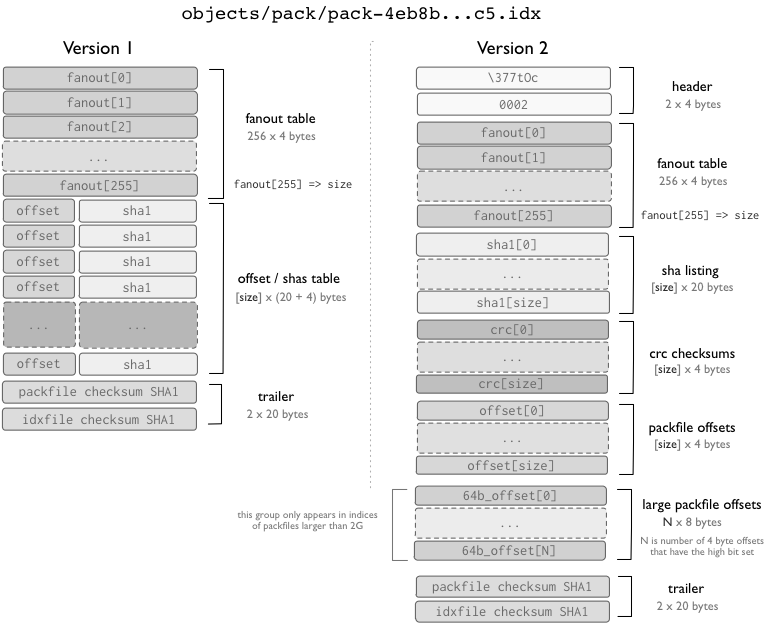
\includegraphics[width=0.80\textwidth]{content/git/packfile-index.png}
\label{fig:packfileindex}
\caption{Packfile Intex}
\end{figure*}

In both formats, the fanout table is simply a way to find the offset of a
particular sha faster within the index file. The offset/sha1[] tables are
sorted by sha1[] values (this is to allow binary search of this table), and
fanout[] table points at the offset/sha1[] table in a specific way (so that
part of the latter table that covers all hashes that start with a given byte
can be found to avoid 8 iterations of the binary search).

In version 1, the offsets and shas are in the same space, where in version two,
there are seperate tables for the shas, crc checksums and offsets. At the end
of both files are checksum shas for both the index file and the packfile it
references.

Importantly, packfile indexes are not neccesary to extract objects from a
packfile, they are simply used to quickly retrieve individual objects from a
pack. The packfile format is used in upload-pack and receieve-pack programs
(push and fetch protocols) to transfer objects and there is no index used then
- it can be built after the fact by scanning the packfile.

\subsubsection{The Packfile Format}
The packfile itself is a very simple format. There is a header, a series of
packed objects (each with it's own header and body) and then a checksum
trailer. The first four bytes is the string 'PACK', which is sort of used to
make sure you're getting the start of the packfile correctly. This is followed
by a 4-byte packfile version number and then a 4-byte number of entries in that
file. In Ruby, you might read the header data like this:
\lstset{basicstyle=\scriptsize, numbers=none, captionpos=b, tabsize=4}
\begin{lstlisting}[caption=,language={ruby},
breaklines=true,label=lst:]
def read_pack_header
  sig = @session.recv(4)
  ver = @session.recv(4).unpack("N")[0]
  entries = @session.recv(4).unpack("N")[0]
  [sig, ver, entries]
end
\end{lstlisting}

After that, you get a series of packed objects, in order of their SHAs which
each consist of an object header and object contents. At the end of the
packfile is a 20-byte SHA1 sum of all the shas (in sorted order) in that
packfile. See figure \ref{fig:packfileformat}

\begin{figure*}[tbp]
\centering
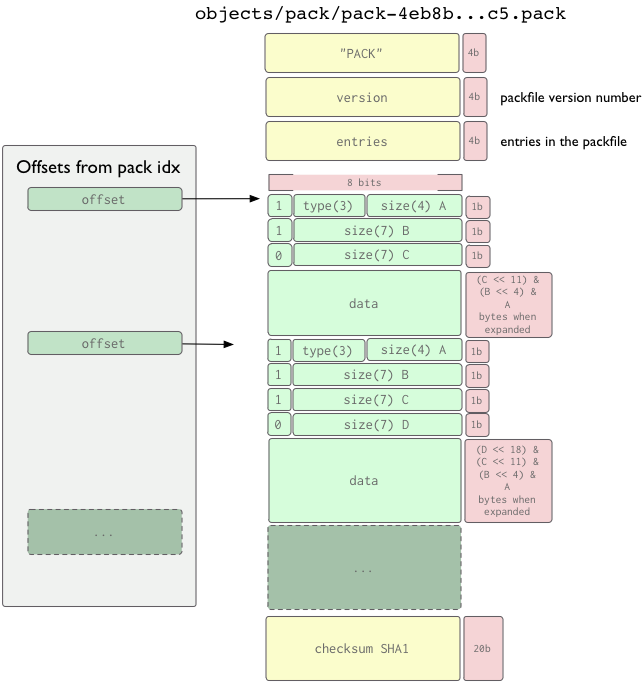
\includegraphics[width=0.80\textwidth]{content/git/packfile-format.png}
\label{fig:packfileformat}
\caption{Packfile format}
\end{figure*}

The object header is a series of one or more 1 byte (8 bit) hunks that specify
the type of object the following data is, and the size of the data when
expanded. Each byte is really 7 bits of data, with the first bit being used to
say if that hunk is the last one or not before the data starts. If the first
bit is a 1, you will read another byte, otherwise the data starts next. The
first 3 bits in the first byte specifies the type of data, according to the
table below.

(Currently, of the 8 values that can be expressed with 3 bits (0-7), 0 (000) is
'undefined' and 5 (101) is not yet used.)

Here, we can see an example of a header of two bytes, where the first specifies
that the following data is a commit, and the remainder of the first and the
last 7 bits of the second specifies that the data will be 144 bytes when
expanded. See figure \ref{fig:packfilelogic}

\begin{figure*}[tbp]
\centering
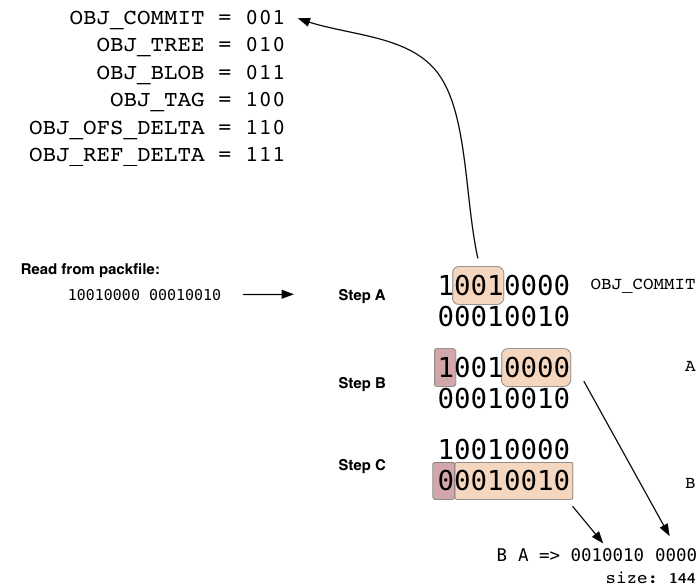
\includegraphics[width=0.80\textwidth]{content/git/packfile-logic.png}
\label{fig:packfilelogic}
\caption{Packfile logic}
\end{figure*}

It is important to note that the size specified in the header data is not the
size of the data that actually follows, but the size of that data when
expanded. This is why the offsets in the packfile index are so useful,
otherwise you have to expand every object just to tell when the next header
starts.

The data part is just zlib stream for non-delta object types; for the two delta
object representations, the data portion contains something that identifies
which base object this delta representation depends on, and the delta to apply
on the base object to resurrect this object.  ref-delta uses 20-byte hash of
the base object at the beginning of data, while ofs-delta stores an offset
within the same packfile to identify the base object. In either case, two
important constraints a reimplementor must adhere to are:

delta representation must be based on some other object within the same
packfile;

the base object must be of the same underlying type (blob, tree, commit or
tag);

\subsection{Raw Git}
Here we will take a look at how to manipulate git at a more raw level, in case
you would like to write a tool that generates new blobs, trees or commits in a
more artificial way. If you want to write a script that uses more low-level git
plumbing to do something new, here are some of the tools you'll need.

\subsubsection{Creating Blobs}
Creating a blob in your Git repository and getting a SHA back is pretty easy.
The git hash-object command is all you'll need. To create a blob object from an
existing file, just run it with the '-w' option (which tells it to write the
blob, not just compute the SHA).
\lstset{basicstyle=\scriptsize, numbers=none, captionpos=b, tabsize=4}
\begin{lstlisting}[caption=,language={bash},
breaklines=true,label=lst:]
$ git hash-object -w myfile.txt
1e4397625791c8ea3bbb5f2279a3

$ git hash-object -w myfile2.txt
ae3185ee32266c860714980dbed7
\end{lstlisting}

The STDOUT output of the command will the the SHA of the blob that was created.

\subsubsection{Creating Trees}
Now lets say you want to create a tree from your new objects. The git mktree
command makes it pretty simple to generate new tree objects from git ls-tree
formatted output. For example, if you write the following to a file named
'/tmp/tree.txt' :
\lstset{basicstyle=\scriptsize, numbers=none, captionpos=b, tabsize=4}
\begin{lstlisting}[caption=,language={bash},
breaklines=true,label=lst:]
100644 blob 1e4397625791c8ea3bbb5f2279a3    file1
100644 blob ae3185ee32266c860714980dbed7    file2
\end{lstlisting}

and then piped that through the git mktree command, Git will write a new tree
to the object database and give you back the new sha of that tree.
\lstset{basicstyle=\scriptsize, numbers=none, captionpos=b, tabsize=4}
\begin{lstlisting}[caption=,language={bash},
breaklines=true,label=lst:]
$ cat /tmp/tree.txt | git mk-tree
fe86d52a66516ace212efa00fe1f
\end{lstlisting}

Then, we can take that and make it a subdirectory of yet another tree, and so
on. If we wanted to create a new tree with that one as a subtree, we just
create a new file (/tmp/newtree.txt) with our new SHA as a tree in it:
\lstset{basicstyle=\scriptsize, numbers=none, captionpos=b, tabsize=4}
\begin{lstlisting}[caption=,language={bash},
breaklines=true,label=lst:]
100644 blob 4664981e4397625791c8ea3bbb5f2279a3    file1-copy
040000 tree ab6a7bfe86d52a66516ace212efa00fe1f    our_files
\end{lstlisting}

and then use git mk-tree again:
\lstset{basicstyle=\scriptsize, numbers=none, captionpos=b, tabsize=4}
\begin{lstlisting}[caption=,language={bash},
breaklines=true,label=lst:]
$ cat /tmp/newtree.txt | git mk-tree
59179bd543a024d6d187692343e2d8ae83
\end{lstlisting}

And we now have an artificial directory structure in Git that looks like this:
\lstset{basicstyle=\scriptsize, numbers=none, captionpos=b, tabsize=4}
\begin{lstlisting}[caption=,language={bash},
breaklines=true,label=lst:]
.
|-- file1-copy
`-- our_files
    |-- file1
    `-- file2

1 directory, 3 files
\end{lstlisting}

without that structure ever having actually existed on disk. Plus, we have a
SHA (5bac6559) that points to it.

\subsubsection{Rearranging Trees}
We can also do tree manipulation by combining trees into new structures using
the index file. As a simple example, let's take the tree we just created and
make a new tree that has two copies of our 5bac6559 tree in it using a
temporary index file. (You can do this by resetting the GIT\_INDEX\_FILE
environment variable or on the command line)

First, we read the tree into our index file under a new prefix using the git
read-tree command, and then write the index contents as a tree using the git
write-tree command:
\lstset{basicstyle=\scriptsize, numbers=none, captionpos=b, tabsize=4}
\begin{lstlisting}[caption=,language={bash},
breaklines=true,label=lst:]
$ export GIT_INDEX_FILE=/tmp/index
$ git read-tree --prefix=copy1/  5bac6559
$ git read-tree --prefix=copy2/  5bac6559
$ git write-tree 
de7625322322382215d9ea78cfe76508c1

$>git ls-tree bb2fa
040000 tree 59179bd543a024d6d187692343e2d8ae83    copy1
040000 tree 59179bd543a024d6d187692343e2d8ae83    copy2
\end{lstlisting}

So now we can see that we've created a new tree just from index manipulation.
You can also do interesting merge operations and such in a temporary index this
way - see the git read-tree docs for more information.

\subsubsection{Creating Commits}
Now that we have a tree SHA, we can create a commit object that points to it.
We can do this using the git commit-tree command. Most of the data that goes
into the commit has to be set as environment variables, so you'll want to set
the following:
\lstset{basicstyle=\scriptsize, numbers=none, captionpos=b, tabsize=4}
\begin{lstlisting}[caption=,language={bash},
breaklines=true,label=lst:]
GIT_AUTHOR_NAME
GIT_AUTHOR_EMAIL
GIT_AUTHOR_DATE
GIT_COMMITTER_NAME
GIT_COMMITTER_EMAIL
GIT_COMMITTER_DATE
\end{lstlisting}

Then you will need to write your commit message to a file or somehow pipe it
into the command through STDIN. Then, you can create your commit object based
on the tree sha we have.
\lstset{basicstyle=\scriptsize, numbers=none, captionpos=b, tabsize=4}
\begin{lstlisting}[caption=,language={bash},
breaklines=true,label=lst:]
$ git commit-tree bb2fa < /tmp/message
a5f85ba5875917319471dfd98dfc636c1dc65650
\end{lstlisting}

If you want to specify one or more parent commits, simply add the shas on the
command line with a '-p' option before each. The SHA of the new commit object
will be returned via STDOUT.

\subsubsection{Updating a Branch Ref}
Now that we have a new commit object SHA, we can update a branch to point to it
if we want to. Lets say we want to update our 'master' branch to point to the
new commit we just created - we would use the git update-ref command:
\lstset{basicstyle=\scriptsize, numbers=none, captionpos=b, tabsize=4}
\begin{lstlisting}[caption=,language={bash},
breaklines=true,label=lst:]
$ git update-ref refs/heads/master a5875917319471dfd98dfc636c1dc65650
\end{lstlisting}

\subsection{Transfer Protocols}
Here we will go over how clients and servers talk to each other to transfer Git
data around.

\subsubsection{Fetching Data over HTTP}
Fetching over an http/s URL will make Git use a slightly dumber protocol. In
this case, all of the logic is entirely on the client side. The server requires
no special setup - any static webserver will work fine if the git directory you
are fetching from is in the webserver path.

In order for this to work, you do need to run a single command on the server
repo everytime anything is updated, though - git update-server-info, which
updates the objects/info/packs and info/refs files to list which refs and
packfiles are available, since you can't do a listing over http. When that
command is run, the objects/info/packs file looks something like this:
\lstset{basicstyle=\scriptsize, numbers=none, captionpos=b, tabsize=4}
\begin{lstlisting}[caption=,language={bash},
breaklines=true,label=lst:]
P pack-ce2bd34abc3d8ebc5922dc81b2e1f30bf17c10cc.pack
P pack-7ad5f5d05f5e20025898c95296fe4b9c861246d8.pack
\end{lstlisting}

So that if the fetch can't find a loose file, it can try these packfiles. The
info/refs file will look something like this:
\lstset{basicstyle=\scriptsize, numbers=none, captionpos=b, tabsize=4}
\begin{lstlisting}[caption=,language={bash},
breaklines=true,label=lst:]
184063c9b594f8968d61a686b2f6052779551613    refs/heads/development
32aae7aef7a412d62192f710f2130302997ec883    refs/heads/master
\end{lstlisting}

Then when you fetch from this repo, it will start with these refs and walk the
commit objects until the client has all the objects that it needs.

For instance, if you ask to fetch the master branch, it will see that master is
pointing to 32aae7ae and that your master is pointing to ab04d88, so you need
32aae7ae. You fetch that object
\lstset{basicstyle=\scriptsize, numbers=none, captionpos=b, tabsize=4}
\begin{lstlisting}[caption=,language={bash},
breaklines=true,label=lst:]
CONNECT http://myserver.com
GET /git/myproject.git/objects/32/aae7aef7a412d62192f710f2130302997ec883 - 200
\end{lstlisting}

and it looks like this:
\lstset{basicstyle=\scriptsize, numbers=none, captionpos=b, tabsize=4}
\begin{lstlisting}[caption=,language={bash},
breaklines=true,label=lst:]
tree aa176fb83a47d00386be237b450fb9dfb5be251a
parent bd71cad2d597d0f1827d4a3f67bb96a646f02889
author Scott Chacon <schacon@gmail.com> 1220463037 -0700
committer Scott Chacon <schacon@gmail.com> 1220463037 -0700

added chapters on private repo setup, scm migration, raw git
\end{lstlisting}

So now it fetches the tree aa176fb8:
\lstset{basicstyle=\scriptsize, numbers=none, captionpos=b, tabsize=4}
\begin{lstlisting}[caption=,language={bash},
breaklines=true,label=lst:]
GET /git/myproject.git/objects/aa/176fb83a47d00386be237b450fb9dfb5be251a - 200
\end{lstlisting}

which looks like this:
\lstset{basicstyle=\scriptsize, numbers=none, captionpos=b, tabsize=4}
\begin{lstlisting}[caption=,language={bash},
breaklines=true,label=lst:]
100644 blob 6ff87c4664981e4397625791c8ea3bbb5f2279a3    COPYING
100644 blob 97b51a6d3685b093cfb345c9e79516e5099a13fb    README
100644 blob 9d1b23b8660817e4a74006f15fae86e2a508c573    Rakefile
\end{lstlisting}

So then it fetches those objects:
\lstset{basicstyle=\scriptsize, numbers=none, captionpos=b, tabsize=4}
\begin{lstlisting}[caption=,language={bash},
breaklines=true,label=lst:]
GET /git/myproject.git/objects/6f/f87c4664981e4397625791c8ea3bbb5f2279a3 - 200
GET /git/myproject.git/objects/97/b51a6d3685b093cfb345c9e79516e5099a13fb - 200
GET /git/myproject.git/objects/9d/1b23b8660817e4a74006f15fae86e2a508c573 - 200
\end{lstlisting}

It actually does this with Curl, and can open up multiple parallel threads to
speed up this process. When it's done recursing the tree pointed to by the
commit, it fetches the next parent.
\lstset{basicstyle=\scriptsize, numbers=none, captionpos=b, tabsize=4}
\begin{lstlisting}[caption=,language={bash},
breaklines=true,label=lst:]
GET /git/myproject.git/objects/bd/71cad2d597d0f1827d4a3f67bb96a646f02889 - 200
\end{lstlisting}

Now in this case, the commit that comes back looks like this:
\lstset{basicstyle=\scriptsize, numbers=none, captionpos=b, tabsize=4}
\begin{lstlisting}[caption=,language={bash},
breaklines=true,label=lst:]
tree b4cc00cf8546edd4fcf29defc3aec14de53e6cf8
parent ab04d884140f7b0cf8bbf86d6883869f16a46f65
author Scott Chacon <schacon@gmail.com> 1220421161 -0700
committer Scott Chacon <schacon@gmail.com> 1220421161 -0700

added chapters on the packfile and how git stores objects
\end{lstlisting}

and we can see that the parent, ab04d88 is where our master branch is currently
pointing. So, we recursively fetch this tree and then stop, since we know we
have everything before this point. You can force Git to double check that we
have everything with the '--recover' option. See git http-fetch for more
information.

If one of the loose object fetches fails, Git will download the packfile
indexes looking for the sha that it needs, then download that packfile.

It is important if you are running a git server that serves repos this way to
implement a post-receive hook that runs the 'git update-server-info' command
each time or there will be confusion. 

\subsubsection{Fetching Data with Upload Pack}
For the smarter protocols, fetching objects is much more efficient. A socket is
opened, either over ssh or over port 9418 (in the case of the git:// protocol),
and the git fetch-pack command on the client begins communicating with a forked
git upload-pack process on the server.

Then the server will tell the client which SHAs it has for each ref, and the
client figures out what it needs and responds with a list of SHAs it wants and
already has.

At this point, the server will generate a packfile with all the objects that
the client needs and begin streaming it down to the client.

Let's look at an example.

The client connects and sends the request header. The clone command
\lstset{basicstyle=\scriptsize, numbers=none, captionpos=b, tabsize=4}
\begin{lstlisting}[caption=,language={bash},
breaklines=true,label=lst:]
$ git clone git://myserver.com/project.git
\end{lstlisting}

produces the following request:
\lstset{basicstyle=\scriptsize, numbers=none, captionpos=b, tabsize=4}
\begin{lstlisting}[caption=,language={bash},
breaklines=true,label=lst:]
0032git-upload-pack /project.git\000host=myserver.com\000
\end{lstlisting}

The first four bytes contain the hex length of the line (including 4 byte line
length and trailing newline if present). Following are the command and
arguments. This is followed by a null byte and then the host information. The
request is terminated by a null byte.

The request is processed and turned into a call to git-upload-pack:
\lstset{basicstyle=\scriptsize, numbers=none, captionpos=b, tabsize=4}
\begin{lstlisting}[caption=,language={bash},
breaklines=true,label=lst:]
$ git-upload-pack /path/to/repos/project.git
\end{lstlisting}

This immediately returns information of the repo:
\lstset{basicstyle=\scriptsize, numbers=none, captionpos=b, tabsize=4}
\begin{lstlisting}[caption=,language={bash},
breaklines=true,label=lst:]
007c74730d410fcb6603ace96f1dc55ea6196122532d HEAD\000multi_ack thin-pack side-band side-band-64k ofs-delta shallow no-progress
003e7d1665144a3a975c05f1f43902ddaf084e784dbe refs/heads/debug
003d5a3f6be755bbb7deae50065988cbfa1ffa9ab68a refs/heads/dist
003e7e47fe2bd8d01d481f44d7af0531bd93d3b21c01 refs/heads/local
003f74730d410fcb6603ace96f1dc55ea6196122532d refs/heads/master
0000
\end{lstlisting}

Each line starts with a four byte line length declaration in hex. The section
is terminated by a line length declaration of 0000.

This is sent back to the client verbatim. The client responds with another
request:
\lstset{basicstyle=\scriptsize, numbers=none, captionpos=b, tabsize=4}
\begin{lstlisting}[caption=,language={bash},
breaklines=true,label=lst:]
0054want 410fcb6603ace96f1dc55ea6196122532d multi_ack side-band-64k ofs-delta
0032want 144a3a975c05f1f43902ddaf084e784dbe
0032want e755bbb7deae50065988cbfa1ffa9ab68a
0032want 2bd8d01d481f44d7af0531bd93d3b21c01
0032want 410fcb6603ace96f1dc55ea6196122532d
00000009done
\end{lstlisting}

The is sent to the open git-upload-pack process which then streams out the
final response:
\lstset{basicstyle=\scriptsize, numbers=none, captionpos=b, tabsize=4}
\begin{lstlisting}[caption=,language={bash},
breaklines=true,label=lst:]
"0008NAK\n"
"0023\002Counting objects: 2797, done.\n"
"002b\002Compressing objects:   0% (1/1177)   \r"
"002c\002Compressing objects:   1% (12/1177)   \r"
"002c\002Compressing objects:   2% (24/1177)   \r"
"002c\002Compressing objects:   3% (36/1177)   \r"
"002c\002Compressing objects:   4% (48/1177)   \r"
"002c\002Compressing objects:   5% (59/1177)   \r"
"002c\002Compressing objects:   6% (71/1177)   \r"
"0053\002Compressing objects:   7% (83/1177)   \rCompressing objects:   8% (95/1177)   \r"
...
"005b\002Compressing objects: 100% (1177/1177)   \rCompressing objects: 100% (1177/1177), done.\n"
"2004\001PACK\000\000\000\002\000\000\n\355\225\017x\234\235\216K\n\302"...
"2005\001\360\204{\225\376\330\345]z2673"...
...
"0037\002Total 2797 (delta 1799), reused 2360 (delta 1529)\n"
...
"<\276\255L\273s\005\001w0006\001[0000"
\end{lstlisting}

See the Packfile chapter previously for the actual format of the packfile data
in the response.

\subsubsection{Pushing Data}
Pushing data over the git and ssh protocols is similar, but simpler. Basically
what happens is the client requests a receive-pack instance, which is started
up if the client has access, then the server returns all the ref head shas it
has again and the client generates a packfile of everything the server needs
(generally only if what is on the server is a direct ancestor of what it is
pushing) and sends that packfile upstream, where the server either stores it on
disk and builds an index for it, or unpacks it (if there aren't many objects in
it)

This entire process is accomplished through the git send-pack command on the
client, which is invoked by git push and the git receive-pack command on the
server side, which is invoked by the ssh connect process or git daemon (if it's
an open push server).

\section{Glossary}
Here we have the meanings of some terms used into Git context.
These terms were entirely copied from Git Glossary.
\definecolor{light-gray}{gray}{0.85}
\subsection*{alternate object database}

\textcolor{light-gray}{Via the alternates mechanism, a repository}

can inherit part of its object database
from another object database, which is called "alternate". 

\subsection*{bare repository}

A bare repository is normally an appropriately

named directory with a `.git` suffix that does not
have a locally checked-out copy of any of the files under
revision control. That is, all of the `git`
administrative and control files that would normally be present in the
hidden `.git` sub-directory are directly present in the
`repository.git` directory instead,
and no other files are present and checked out. Usually publishers of
public repositories make bare repositories available.
blob object

Untyped object, e.g. the contents of a file.

branch

A "branch" is an active line of development. The most recent

commit on a branch is referred to as the tip of
that branch.  The tip of the branch is referenced by a branch
head, which moves forward as additional development
is done on the branch.  A single git
repository can track an arbitrary number of
branches, but your working tree is
associated with just one of them (the "current" or "checked out"
branch), and HEAD points to that branch.
cache

Obsolete for: index.

chain

A list of objects, where each object in the list contains

a reference to its successor (for example, the successor of a
commit could be one of its parents).
changeset

BitKeeper/cvsps speak for "commit". Since git does not

store changes, but states, it really does not make sense to use the term
"changesets" with git.
checkout

The action of updating all or part of the

working tree with a tree object
or blob from the
object database, and updating the
index and HEAD if the whole working tree has
been pointed at a new branch.
cherry-picking

In SCM jargon, "cherry pick" means to choose a subset of

changes out of a series of changes (typically commits) and record them
as a new series of changes on top of a different codebase. In GIT, this is
performed by the "git cherry-pick" command to extract the change introduced
by an existing commit and to record it based on the tip
of the current branch as a new commit.
clean

A working tree is clean, if it

corresponds to the revision referenced by the current
head. Also see "dirty".
commit

As a noun: A single point in the

git history; the entire history of a project is represented as a
set of interrelated commits.  The word "commit" is often
used by git in the same places other revision control systems
use the words "revision" or "version".  Also used as a short
hand for commit object.
As a verb: The action of storing a new snapshot of the project's

state in the git history, by creating a new commit representing the current
state of the index and advancing HEAD
to point at the new commit.
commit object

An object which contains the information about a

particular revision, such as parents, committer,
author, date and the tree object which corresponds
to the top directory of the stored
revision.
core git

Fundamental data structures and utilities of git. Exposes only limited

source code management tools.
DAG

Directed acyclic graph. The commit objects form a

directed acyclic graph, because they have parents (directed), and the
graph of commit objects is acyclic (there is no chain
which begins and ends with the same object).
dangling object

An unreachable object which is not

reachable even from other unreachable objects; a
dangling object has no references to it from any
reference or object in the repository.
detached HEAD

Normally the HEAD stores the name of a

branch.  However, git also allows you to check out
an arbitrary commit that isn't necessarily the tip of any
particular branch.  In this case HEAD is said to be "detached".
dircache

You are waaaaay behind. See index.

directory

The list you get with "ls" :-)

dirty

A working tree is said to be "dirty" if

it contains modifications which have not been committed to the current
branch.
ent

Favorite synonym to "tree-ish" by some total geeks. See

Middle-earth for an in-depth
explanation. Avoid this term, not to confuse people.
evil merge

An evil merge is a merge that introduces changes that

do not appear in any parent.
fast forward

A fast-forward is a special type of merge where you have a

revision and you are "merging" another
branch's changes that happen to be a descendant of what
you have. In such these cases, you do not make a new merge
commit but instead just update to his
revision. This will happen frequently on a
tracking branch of a remote
repository.
fetch

Fetching a branch means to get the

branch's head ref from a remote
repository, to find out which objects are
missing from the local object database,
and to get them, too.  See also git fetch.
file system

Linus Torvalds originally designed git to be a user space file system,

i.e. the infrastructure to hold files and directories. That ensured the
efficiency and speed of git.
git archive

Synonym for repository (for arch people).

grafts

Grafts enables two otherwise different lines of development to be joined

together by recording fake ancestry information for commits. This way
you can make git pretend the set of parents a commit has
is different from what was recorded when the commit was
created. Configured via the `.git/info/grafts` file.
hash

In git's context, synonym to object name.

head

A named reference to the commit at the tip of a

\scriptsize
\begin{verbatim}
$GIT_DIR/refs/heads/, except when using packed refs. (See
git pack-refs.)
\end{verbatim}
\normalsize

HEAD

The current branch. In more detail: Your working tree is normally derived

from the state of the tree referred to by HEAD.  HEAD is a reference to one
of the heads in your repository, except when using a detached HEAD, in which
case it may reference an arbitrary commit.
head ref

A synonym for head.

hook

During the normal execution of several git commands, call-outs are made
\scriptsize
\begin{verbatim}
to optional scripts that allow a developer to add functionality or
checking. Typically, the hooks allow for a command to be pre-verified
and potentially aborted, and allow for a post-notification after the
operation is done. The hook scripts are found in the
`$GIT_DIR/hooks/` directory, and are enabled by simply
removing the `.sample` suffix from the filename. In earlier versions
of git you had to make them executable.
\end{verbatim}
\normalsize

index

A collection of files with stat information, whose contents are stored

as objects. The index is a stored version of your
working tree. Truth be told, it can also contain a second, and even
a third version of a working tree, which are used
when merging.
index entry

The information regarding a particular file, stored in the

index. An index entry can be unmerged, if a
merge was started, but not yet finished (i.e. if
the index contains multiple versions of that file).
master

The default development branch. Whenever you

create a git repository, a branch named
"master" is created, and becomes the active branch. In most
cases, this contains the local development, though that is
purely by convention and is not required.
merge

As a verb: To bring the contents of another

branch (possibly from an external
repository) into the current branch.  In the
case where the merged-in branch is from a different repository,
this is done by first fetching the remote branch
and then merging the result into the current branch.  This
combination of fetch and merge operations is called a
pull.  Merging is performed by an automatic process
that identifies changes made since the branches diverged, and
then applies all those changes together.  In cases where changes
conflict, manual intervention may be required to complete the
merge.
As a noun: unless it is a fast forward, a

successful merge results in the creation of a new commit
representing the result of the merge, and having as
parents the tips of the merged branches.
This commit is referred to as a "merge commit", or sometimes just a
"merge".
object

The unit of storage in git. It is uniquely identified by the

SHA1> of its contents. Consequently, an
object can not be changed.
object database

Stores a set of "objects", and an individual object is
\scriptsize
\begin{verbatim}
identified by its object name. The objects usually
live in `$GIT_DIR/objects/`.
\end{verbatim}
\normalsize

object identifier

Synonym for object name.

object name

The unique identifier of an object. The hash

of the object's contents using the Secure Hash Algorithm
1 and usually represented by the 40 character hexadecimal encoding of
the hash of the object.
object type

One of the identifiers "commit", "tree", "tag" or "blob" describing the

type of an object.
octopus

To merge more than two branches. Also denotes an

intelligent predator.
origin

The default upstream repository. Most projects have

at least one upstream project which they track. By default
'origin' is used for that purpose. New upstream updates
will be fetched into remote tracking branches named
origin/name-of-upstream-branch, which you can see using
"`git branch -r`".
pack

A set of objects which have been compressed into one file (to save space

or to transmit them efficiently).
pack index

The list of identifiers, and other information, of the objects in a

pack, to assist in efficiently accessing the contents of a
pack.
parent

A commit object contains a (possibly empty) list

of the logical predecessor(s) in the line of development, i.e. its
parents.
pickaxe

The term pickaxe refers to an option to the diffcore

routines that help select changes that add or delete a given text
string. With the `--pickaxe-all` option, it can be used to view the full
changeset that introduced or removed, say, a
particular line of text. See git diff.
plumbing

Cute name for core git.

porcelain

Cute name for programs and program suites depending on

core git, presenting a high level access to
core git. Porcelains expose more of a SCM
interface than the plumbing.
pull

Pulling a branch means to fetch it and

merge it.  See also git pull.
push

Pushing a branch means to get the branch's

head ref from a remote repository,
find out if it is a direct ancestor to the branch's local
head ref, and in that case, putting all
objects, which are reachable from the local
head ref, and which are missing from the remote
repository, into the remote
object database, and updating the remote
head ref. If the remote head is not an
ancestor to the local head, the push fails.
reachable

All of the ancestors of a given commit are said to be

"reachable" from that commit. More
generally, one object is reachable from
another if we can reach the one from the other by a chain
that follows tags to whatever they tag,
commits to their parents or trees, and
trees to the trees or blobs
that they contain.
rebase

To reapply a series of changes from a branch to a

different base, and reset the head of that branch
to the result.
ref

A 40-byte hex representation of a SHA1 or a name that
\scriptsize
\begin{verbatim}
denotes a particular object. These may be stored in
`$GIT_DIR/refs/`.
\end{verbatim}
\normalsize

reflog

A reflog shows the local "history" of a ref. In other words,
\scriptsize
\begin{verbatim}
it can tell you what the 3rd last revision in _this_ repository
was, and what was the current state in _this_ repository,
yesterday 9:14pm.  See git reflog for details.
\end{verbatim}
\normalsize

refspec

A "refspec" is used by fetch and

push to describe the mapping between remote
ref and local ref. They are combined with a colon in
the format <src>:<dst>, preceded by an optional plus sign, +.
For example: `git fetch $URL
refs/heads/master:refs/heads/origin` means "grab the master
branch head from the $URL and store
it as my origin branch head". And `git push
$URL refs/heads/master:refs/heads/to-upstream` means "publish my
master branch head as to-upstream branch at $URL". See also
git push.
repository

A collection of refs together with an

object database containing all objects
which are reachable from the refs, possibly
accompanied by meta data from one or more porcelains. A
repository can share an object database with other repositories
via alternates mechanism.
resolve

The action of fixing up manually what a failed automatic

merge left behind.
revision

A particular state of files and directories which was stored in the

object database. It is referenced by a
commit object.
rewind

To throw away part of the development, i.e. to assign the

head to an earlier revision.
SCM

Source code management (tool).

SHA1

Synonym for object name.

shallow repository

A shallow repository has an incomplete

history some of whose commits have parents cauterized away (in other
words, git is told to pretend that these commits do not have the
parents, even though they are recorded in the commit
object). This is sometimes useful when you are interested only in the
recent history of a project even though the real history recorded in the
upstream is much larger. A shallow repository
is created by giving the `--depth` option to git clone, and
its history can be later deepened with git fetch.
symref

Symbolic reference: instead of containing the SHA1

id itself, it is of the format 'ref: refs/some/thing' and when
referenced, it recursively dereferences to this reference.
'HEAD' is a prime example of a symref. Symbolic
references are manipulated with the git symbolic-ref
command.
tag

A ref pointing to a tag or

\scriptsize
\begin{verbatim}commit object. In contrast to a head,
a tag is not changed by a commit. Tags (not
tag objects) are stored in `$GIT_DIR/refs/tags/`. A
git tag has nothing to do with a Lisp tag (which would be
called an object type in git's context). A
tag is most typically used to mark a particular point in the
commit ancestry chain.
\end{verbatim}
\normalsize

tag object

An object containing a ref pointing to

another object, which can contain a message just like a
commit object. It can also contain a (PGP)
signature, in which case it is called a "signed tag object".
topic branch

A regular git branch that is used by a developer to

identify a conceptual line of development. Since branches are very easy
and inexpensive, it is often desirable to have several small branches
that each contain very well defined concepts or small incremental yet
related changes.
tracking branch

A regular git branch that is used to follow changes from

another repository. A tracking
branch should not contain direct modifications or have local commits
made to it. A tracking branch can usually be
identified as the right-hand-side ref in a Pull:
refspec.
tree

Either a working tree, or a tree object together with the dependent

blob and tree objects (i.e. a stored representation of a working tree).
tree object

An object containing a list of file names and modes along

with refs to the associated blob and/or tree objects. A
tree is equivalent to a directory.
tree-ish

A ref pointing to either a commit object, a tree object, or a tag

object pointing to a tag or commit or tree object.
unmerged index

An index which contains unmerged

index entries.
unreachable object

An object which is not reachable from a

branch, tag, or any other reference.
working tree

The tree of actual checked out files. The working tree is

normally equal to the HEAD plus any local changes
that you have made but not yet committed.

